%----------
%	DOKUMENTUAREN KONFIGURAZIOA
%----------

% Dokumentu mota definitu eta pakete batzuk gehituko ditugu (\usepackage{package}), LaTeX-i funtzioak gehitzeko.
\documentclass[12pt]{report} % 12 puntuko letra
\renewcommand{\baselinestretch}{1.5} % lerro-arteko espazioa 1,5ekoa
\parskip=6pt % 6 puntuko lerro saltoa

% MARGINAK: 2,54 cm goian, behean eta aldeetan.
\usepackage[a4paper,vmargin=2.54cm,hmargin=2.54cm,headsep=2cm]{geometry}
\usepackage{changepage}

% EDUKIAK
\usepackage{titling}

% KOLOREAK: portada eta listetako kodeentzako.
\usepackage[table]{xcolor}
\definecolor{}{RGB}{0,0,0}
\definecolor{gray97}{gray}{.97}
\definecolor{gray75}{gray}{.75}
\definecolor{gray56}{gray}{.56}

% PDF-A SORTZEKO --Metadatuak sortzeko beharrezkoa. <izena>.tex fitxategiaren alboan izen bereko .xmpdata fitxategi bat egon behar da.
\usepackage[a-1b]{pdfx}

% LINKAK
\usepackage{hyperref}
\hypersetup{colorlinks=true,
	linkcolor=black, % dokumentura linkak (aurkibidea, ...) beltzez
	citecolor=black, % zitak ere beltzez
	urlcolor=blue} % kanpora doazen linkak urdinez

% MATEMATIKAKO EXPRESIOAK ERABILTZEKO
\usepackage{amsmath,amssymb,amsfonts,amsthm}
\usepackage{txfonts}
\usepackage[T1]{fontenc}
\usepackage[utf8]{inputenc}

% HIZKUNTZA
\usepackage[basque]{babel}
\usepackage[babel, spanish=spanish]{csquotes}
\AtBeginEnvironment{quote}{\small}

% ORRI OINA
\usepackage{fancyhdr}
\pagestyle{fancy}
\fancyhf{}
\renewcommand{\headrulewidth}{0pt}
\renewcommand{\footrulewidth}{0.75pt}
\renewcommand{\footrule}{\hbox to\headwidth{\color{gray56}\leaders\hrule height \footrulewidth\hfill}}
\rfoot{\thepage}
\fancypagestyle{plain}{\pagestyle{fancy}}

% TITULOEN EZARPENAK
\usepackage{titlesec}
%\titleformat{command}{format}{label}{sep}{before-code}[after-code]
\usepackage{titletoc}
%\usepackage{tocloft}

%%% Chapter
\titleformat{\chapter}
{\bfseries\framebox[\linewidth][l]}
{\thechapter.}
{5pt}
{\MakeUppercase}
{}

% Aurkibideendako bakarrik erabilia
\titleformat{name=\chapter,numberless}
{\large\bfseries\filcenter}
{}
{5pt}
{\MakeUppercase}
{}

\titlespacing{\chapter}{0pt}{0pt}{*3}
\titlecontents{chapter}
[0pt]
{}
{\contentsmargin{0pt}\thecontentslabel.\enspace\uppercase}
{\contentsmargin{0pt}\uppercase}
{\titlerule*[.7pc]{.}\contentspage}
%%% Section
\titleformat{\section}
{\normalsize\bfseries}
{\thesection.}
{5pt}
{}

\titlecontents{section}
[5pt]
{}
{\contentsmargin{0pt}\thecontentslabel.\enspace}
{\contentsmargin{0pt}}
{\titlerule*[.7pc]{.}\contentspage}
%%% Subsection
\titleformat{\subsection}
{\normalsize\bfseries\itshape}
{\thesubsection.}
{5pt}
{}

\titlecontents{subsection}
[10pt]
{}
{\contentsmargin{0pt}
	\thecontentslabel.\enspace}
{\contentsmargin{0pt}}
{\titlerule*[.7pc]{.}\contentspage}
%%% Subsubsection
\titleformat{\subsubsection}
{\normalsize}
{\thesubsubsection.}
{5pt}
{\underline}

\titlecontents{subsubsection}
[10pt]
{}
{\contentsmargin{0pt}
	\thecontentslabel.\enspace}
{\contentsmargin{0pt}}
{\titlerule*[.7pc]{.}\contentspage}

% NORBERAREN EZARPENAK
\setcounter{tocdepth}{3}
\setcounter{secnumdepth}{4}

\titleformat{\paragraph}
{\normalfont\normalsize\bfseries}{\theparagraph}{1em}{}
\titlespacing*{\paragraph}
{0pt}{3.25ex plus 1ex minus .2ex}{1.5ex plus .2ex}

\usepackage{pdfpages}

% TAULAK
\usepackage{multirow} % zeldak linkatzea ahalbidetzen du
\usepackage{caption} % tituluak konfiguratu ahal izateko
\usepackage{floatrow} % tituluak alineatzeko hau erabiltzen da
\DeclareCaptionLabelFormat{aurretik}{\textbf{#2. #1. }}
\usepackage{makecell}
\renewcommand{\cellalign}{tl}

% Taularen diseinua
\captionsetup[table]{
	position=top,
	name=Taula,
	singlelinecheck=off,
	labelsep=none,
	labelformat=aurretik,
	justification=raggedright,
}

% IRUDIAK.
\usepackage{graphicx}
\graphicspath{{images/}} % irudien karpetaren erroa

% Irudien diseinua
\captionsetup[figure]{
	position=top,
	name=Irudia,
	singlelinecheck=off,
	labelsep=none,
	labelformat=aurretik,
	justification=raggedright,
}

% ORRI OINEKO NOTAK
\usepackage{chngcntr} % numerazio kontinuoa erabiltzeko
\counterwithout{footnote}{chapter}


%BIBLIOGRAFÍA - Aldaketak eginez gero ez bada ezer gertatzen, artxibo auxiliarrak borratu eta orden honetan konpilatu fitxategia: 1. COMPILAR-BIBLIOGRAFIA 2. COMPILAR

% Biber-ekin bibliografia sortzeko eta textu editorea konfiguratzeko hemen daukazu informazio gehiago: http://tex.stackexchange.com/questions/154751/biblatex-with-biber-configuring-my-editor-to-avoid-undefined-citations , https://www.overleaf.com/learn/latex/Bibliography_management_in_LaTeX y en http://www.ctan.org/tex-archive/macros/latex/exptl/biblatex-contrib

% APA BIBLIOGRAFIARAKO AUKERAK
\usepackage[backend=biber, style=apa, isbn=false, sortcites, maxbibnames=5, minbibnames=1, urldate=ymd]{biblatex} % APA zientzia sozialetarako gomendatzen den estiloak: "maxbibnames" autore kopurutik gora dagoenean "minbibnames" kopuruan etengo du lista, eta "et al." gehituko du.
% \DeclareLanguageMapping{basque}{bibliography/basque-apa} % basque-apa ez dagoenez, guk sortua erabiliko dugu

\DeclareLanguageMapping{basque}{spanish-apa} % basque-apa ez dagoenez, ingelesa erabiliko dugu

\DefineBibliographyStrings{basque}{%
  jourarticle      = {artikulua},
  article          = {artikulua},
  supplement       = {eranskina},
  part             = {atal},
  january          = {urtarrilaren},
  february         = {otsailaren},
  march            = {martxoaren},
  april            = {apirilaren},
  may              = {maiatzaren},
  june             = {ekainaren},
  july             = {uztailaren},
  august           = {abuztuaren},
  september        = {irailaren},
  october          = {urriaren},
  november         = {azaroaren},
  december         = {abenduaren},
  nodate           = {d\adddot g\adddot},
  page             = {Orrialdea},
  pages            = {Orrialdeak},
  and              = {eta},
  andothers        = {et\space al\adddot},
  retrieved        = {Azken\space aldiz\space ikusia},
  from             = {eskuragarri\space hemen:},
}

\addbibresource{bibliography/bibliography.bib} % artxiboari bibliography.bib deitu, eta bibliografia bertan sartu

% ENUMERATUAK
\renewcommand{\labelenumii}{\theenumii}
\renewcommand{\theenumii}{\theenumi.\arabic{enumii}.}

% EURO
\usepackage{eurosym} % euroaren sinboloa erabili ahal izateko

% GOIBURU ETA ORRI OINA
\usepackage{fancyhdr}

\pagestyle{fancy}
\fancyhf{}
\lhead{
\includegraphics[width=3.59cm]{images/orri_burua.png}}
\rfoot{\thepage}

%----------------
%	DOKUMENTUA
%----------------

\begin{document}
%\pagenumbering{Roman} % Lanaren gorputza baino lehenagoko orrietarako letra erromatarrak erabiliko dira

%-----------
%	AZALA
%-----------
\begin{titlepage}
	
\includepdf[pages=-]{resources/Portada}
\end{titlepage}
\color{black}

\newpage %orri hutsa
\thispagestyle{empty}
\mbox{}


%----------
%	LABURPENA ETA HITZ GAKOAK (ABSTRACT)
%----------

\renewcommand{\abstractname}{\large\bfseries\filcenter\uppercase{Laburpena}}
\begin{abstract}
	\thispagestyle{plain}
    \setcounter{page}{4}

	Master Bukaerako Lan (MBL) honen xedea ikastetxeetan burujabetza digitalaren bidean urratsak ematen lagunduko duen formakuntza saio bat diseinatzea da. Horretarako, irakasle jarduna komunitate baten baitan ulertu eta ikastetxeko ekosistema indartzeko helburuz, Praktika Komunitate Profesionalen (PKP) markoan oinarritutako formakuntza saioa proposatzen da. Dokumentu honen hasieran problematika honen aurrean egin diren aurrekariak azaltzen dira; honekin lotuta, oinarri teorikoak zehazten dira; eta azkenik, finkatutako helburuak betetzeko formakuntza saioa diseinatzen da.
	
	Formakuntza saioak landuko diren problematika desberdinak, helburuak, edukiak eta sekuentziazio bat ditu zehaztuta. Hortaz gain, erabiliko den metodologia zehazten da eta beharrezko baliabideak definitzen dira. Azkenik, PKP oinarrien baitan, formakuntzaren feedback eta norberaren autoebaluazioa egitea proposatzen da, jakintzak ikastetxean hedatzeko lagungarria izango dena.
	\begin{flushright}
		\textbf{Euskara}
	\end{flushright}
	
	\vspace{1.5\baselineskip}
	
	\textbf{Hitz gakoak:}\par
	Burujabetza Digitala; Formakuntza Saioa; Baliabide Digital Libreak; GAFAM; Zientzia, Teknologia eta Gizartea; PKP\par
	
	\vfill
\end{abstract}
\renewcommand{\abstractname}{\large\bfseries\filcenter\uppercase{Abstract}}
\begin{abstract}
	\thispagestyle{plain}
    \setcounter{page}{5}
	
	The purpose of this Final Master's Thesis (FMT) is to design a training course that will help schools in their way to digital autonomy. Understanding teaching as a community job, and to strengthen the school ecosystem, Professional Learning Community (PLC) framework is chosen for this course. By the start of the document, the background of this context can be read; it follows with the theoretical framework; and finally, and to reach the goals of this thesis, the training course can be found.
	
	The training course details the description of the problems, the goals, the contents and the scheduling. It also defines the methodology to be used and the resources required. Last, and following PLC basis, it is proposed to feedback the course and realize an auto-evaluation, that will be helpful to spread the knowledge upon the school.
	\begin{flushright}
		\textbf{English}
	\end{flushright}

	\vspace{1.5\baselineskip}

	\textbf{Keywords:}\par
	Digital Autonomy; Training Course; Open Digital Resources; GAFAM; Science, Technology and Society, PLC\par

	\vfill
\end{abstract}

\newpage %orri hutsa
\thispagestyle{empty}
\mbox{}

%----------
%	Eskerrak
%----------	
%\chapter*{Eskerrak}
%
%\setcounter{page}{5}

%Norbait eskertu nahi gero, idatzi hemen.

%\vfill

%\newpage % orri hutsa
%\thispagestyle{empty}
%\mbox{}

%----------
%	AURKIBIDEA
%----------

\setcounter{page}{6}
\newpage
%--
% Aurkibide orokorra
%-
%\renewcommand{\contentsname}{\hfill\large\bfseries\uppercase{Gaien aurkibidea}\hfill}

\thispagestyle{fancy}
\tableofcontents
\newpage % orri hutsa

%--
% Irudien aurkibidea (egon ezean, komentatu hurrengo lerroak)
%-
%\renewcommand{\listfigurename}{\hfill\large\bfseries\uppercase{Irudien zerrenda}\hfill}

\thispagestyle{fancy}
\listoffigures
\newpage % orri hutsa

%--
% Taulen aurkibidea (egon ezean, komentatu hurrengo lerroak)
%-
%\renewcommand{\listtablename}{\hfill\large\bfseries\uppercase{Taulen zerrenda}\hfill}

\thispagestyle{fancy}
\listoftables
\newpage % orri hutsa

\thispagestyle{empty}
\mbox{}


%----------
%	LANA
%----------
\clearpage
\pagenumbering{arabic} % publikazio osorako zenbaki arabigoak erabiliko dira
\setcounter{page}{1}

%%%%%%%%%%%%%
%% SARRERA %%
%%%%%%%%%%%%%
\chapter{Sarrera}\label{cha:sarrera}
Bigarren Hezkuntzako Master amaierako lan hau irakasleen formakuntza saio bat diseinatzean datza, Praktika Komunitate Profesionalaren markoaren baitan. Gaur egun bizi garen gizartea, etengabeko aldaketek eta garapen zientifiko eta teknologikoak ezaugarritzen dute. Testuinguru honetan, nahiz eta, garapen honek hobekuntzak ekarri egunerokotasuneko bizitzetara, herrialde aberatsen eta pobreen arteko arrakala asko handitu du adibidez, eta baliabide teknologiko hauen parte handi bat multinazional gutxi batzuen esku dago.

Egoera honek zuzenean eragiten du hezkuntza sisteman ere, bertan zabalduena dauden baliabide teknologikoak GAFAM (\ref{sec:gafam}. atalean azalduko dena) enpresen esku baitaude. Modu horretan, alde batik, enpresek hezkuntza sisteman parte hartzen dute eta horrek datu kantitate handietara sarbidea bermatzen die, ondoren datu horiekin soilik multinazional handientzako mesedegarriak izango diren negozio berriak sortzeko. Beste alde batetik, ikasle eta orohar erabiltzaileen pribatutasuna eta norbere datuen kontrola erabat galtzen da.

Honen aurrean, beharrezkoa da inguratzen gaituen errealitatearekiko kontzientzia hartu eta ikuspegi kritiko batetik aztertzea egoera, ondoren egoera honi aurre egingo dioten planteamenduak garatzeko. Horretarako, hezkuntzaren eremua sektore klabe moduan identifikatzen da, hein handi batean aldaketak gauzatzeko baldintzak sortzeko gaitasuna dagoelako bertatik, egungo ikasleei beste balio batzuetan hezi eta haziz.

Baina hau guztia aurrera eramateko ezinbestekoa da irakaslegoak honekiko prestakuntza eduki eta kontziente izatea. Hori dela eta, irakasleentzako diseinatu den formakuntza saio honek hiru alderdi nagusi lantzea du helburu: GAFAM enpresek hezkuntzan aurrera eramaten duten esku- hartzea ezaugarritzea, egoera honi aurre egin eta burujabetza digitalera bidean martxan dauden proiektuen oinarriak azaldu eta beraien planteamenduak ezagutzera ematea eta baliabide teknologiko libreak ezagutarazi, hauek aurkitzen jakiteko gaitasunak eskuratu eta hauen erabileran irakasleak trebatzea.

Dokumentuaren egiturari dagokionez, hasteko eta behin, lanaren helburuak definitu dira eta proiektuaren justifikazioa egin da. Jarraian, irakasleen formakuntzak izango dituen oinarri teorikoak garatu dira, marko teorikoaren atalaren barruan. Ondoren, Praktika Komunitate Profesionalaren markoan oinarritzen den formakuntza saioa aurkezten da.

Azkenik, garatutako formakuntza saiotik eta oinarri teorikoetatik ateratako hainbat ondorio aurkezten dira eta etorkizunean garatu daitezkeen lan lerro posibleak definitu dira.\\

%%%%%%%%%%%%%%%
%% HELBURUAK %%
%%%%%%%%%%%%%%%
{\let\clearpage\relax \chapter{Helburuak}\label{cha:helburuak}}

Bi helburu mota bereizi daitezke. Lehenik eta behin, master bukaerako lan honen helburu orokorrak finkatuko dira. Ondoren, eta garatu den formakuntza saioaren helburuak finkatuko dira.

Hasteko, eta txostenaren helburuak begiratuz, hainbat puntu azpimarra daitezke:
\begin{itemize}
    \item DigCompEdu (\ref{subsec:digcompedu}. atalean sakonduko dena) markoan oinarrituta EAEko ikastetxeetako digitalizazio maila aztertzea.
    \item Hezkuntzaren sektorean interesa erakutsi duten enpresen interes eta helburuak kritikoki aztertzea.
    \item Burujabetza digitalaren inguruko hausnarketa egitea eta kontzientzia garatzea.
    \item Baliabide libreak identifikatzea eta horietan trebatzea.
    \item Irakasleentzako formakuntza saio bat diseinatzea.
\end{itemize}

Honekin jarraituz, MBLaren helburu nagusia irakasleentzako formakuntza saio bat burutzea da. Goian dauden helburuak irakasle komunitatera hedatzeko beharra dagoela identifikatu da, eta formakuntza saioez baliatuz egin behar dela uste da. Beraz, saio honek bete behar dituen helburuak honako hauek dira:
\begin{itemize}
    \item Derrigorrezko Bigarren Hezkuntzako (DBH) eta Batxilergoko irakasleentzat diseinatzea.
    \item Metodologia aktiboak erabiltzea, kurtsoaren eraginkortasuna areagotzeko.
    \item PKP markoan oinarritutako irakasle lantaldea eratzea.
    \item Baliabide digitalak erabiltzea, ahal den heinean, multinazional handien \textit{software}tik\footnote{Programa informatiko.} kanpo.
    \item Irakasle bakoitzak bere buruaren progresuaren gaineko hausnarketa egitea, autoebaluazioaren bidez.
    \item Ikastetxean aldaketak bultzatzeko, eskuratutako jakintzak komunitate guztira zabaltzea.
    \item Etengabeko hobekuntza ardatz, irakasleek jasotako formakuntza saioaren gaineko ebaluazioa egitea.
\end{itemize}

Helburu hauek bete diren dokumentuaren amaieran ondorioztatuko da, \ref{cha:ondorioak}. atalean.\\

%%%%%%%%%%%%%%%%%%%
%% JUSTIFIKAZIOA %%
%%%%%%%%%%%%%%%%%%%
{\let\clearpage\relax \chapter{Justifikazioa}\label{cha:justifikazioa}}
Gizarte mailan, transformazio teknologiko eta digitalak presentzia handia hartu du azken urteotan eta honek bizitzako esparru desberdinetan gaur egun arte izan duen eragina kontuan hartuta, inpaktu handia izango du etorkizun laburrean.

Izan ere, eskola ez da ekosistema itxi bat, baizik gizarte eta ekosistema komun baten barruan dago: horregatik, zergatik eta zertarako hezkuntza teknologiko-zientifiko-matematikoari galdera erantzunez, hainbat erronka azaleratzen dira gizarte mailan. Hauen artean, aipatutako transformazio teknologiko eta digitalak, hezkuntza teknologikoan eragin zuzena duen problematika dago. Teknologiaren garapen ikaragarria, oso denbora laburrean ematen ari da eta hezkuntza sisteman aldaketak nabarmenak dira. Multinazional handiek teknologia digitalen merkatua monopolizatuta dute eta hezkuntza sistemaren parte dira jada. Horregatik, hezkuntza sisteman dugun erronka nagusienetako bat burujabetza digitalerako pausuak ematea da.

\citeauthor{ehd2021manifestua}-k (\citeyear{ehd2021manifestua}), XX. mende amaieratik hezkuntza sakoneko eraldaketa batean murgildurik dagoela dio. Digitalizazioa eskoletara iristeak prozesu hau areagotu du eredu zaharraren pilareak kolpatzen dituen heinean. baina erantzuten dituenak baino galdera gehiago sortzen ditu, Pandemiarekin hezkuntzaren beharrak aztertuz baina, galdera gehiago sortzen ditu: presentzialtasunaren garrantzia, ingurune digitalaren jabea nor izan behar den, nola bermatzen diren hezkuntzarako eskubidea eta abar. Digitalizazioak erronka zaharrei erantzuteko galdera berriak planteatzen ditu hezkuntzan ere.

Azken finean, helburua, teknologia eta ikuspuntu teknologikoa gizartearen zerbitzura egongo dena, pertsonen bizitzak hobetzeko erabiltzea da. Teknologia ez baita neutrala, teknologia guk (gizarteak) egiten dugu eta hezkuntza enpresa multinazionalen eskuetan utzi dugun honetan, hauek hezkuntzara hurbiltzeaz gain, haien ekosistema digitalak ikastetxeetan infiltratu dira. 

Honi mugak jarri eta burujabetza digitalaren bidean ikastetxeek aurrera pausuak emateko, beharrezkoa ikusten dugu irakasleak, herritar ororen moduan, konpetentzia teknologiko-digitaletan oinarrizko ezagutzak izatea eta hauetan eguneratuta egotea. Trebezietatik haratago, ikuspegi kritiko bat garatu eta digitalizazioaren nolakotasunean fokua jartzea, “etikoa, arduratsua, eraginkorra eta euskalduna” hain zuzen ere.

Gauzak horrela, hezkuntzaren gaur egungo eta etorkizuneko erronka nagusiei erantzuteko irakasleak prestatu behar ditugu. Horregatik, Master Bukaerako Lan honetan PKP markoan oinarritutako formakuntza saio baten diseinua egitea erabaki da.

\chapter{Aurrekariak}\label{cha:aurrekariak}

Gaur egungo egoera ulertzeko, aro garaikidean eman diren hainbat fenomeno ulertzea beharrezkoak dira. Aldi berean, tesi honek defendatzen duen argumentuak izan dituen estatu eta Europa mailako proiektuak aztertuko dira jarraian datorren atalean.

\section{Globalizazioa}\label{sec:globalizazioa}
Globalizazioa fenomeno tekniko bat da eta sistema kapitalistak gaur egun hartzen duen forma konkretua. Jadanik 1848an Marx eta Engels-ek garatutako Manifestu Komunistan aurreikusten zuten globalizazioaren fenomenoa ekoizleen internazionalizazioaren bidetik (\cite{prieto2005globalizacion}). Baina XX. mende bukaeran azaleratu zen globalizazioaren gaia modu sakonago batean. Teknologiaren garapen sakon bat ematen da eta mundua gero eta txikiago bihurtu. Hau da, globalizazioaren eraginez izugarri hazi da merkantzien, kapitalen eta pertsonen mundu mailako fluxua, munduko edozein produktu eskuragarri jarriz. Honen ondorioz, beste herrialdeekiko dependentzia asko handitu da produktu asko inportatzen direlako. Honen adibide garbia, pandemia hasieran musukoen hornikuntzan kanpoko herrialdeekiko zegoen dependentzia da.

Fenomenok honek, bizitzako esfera guztietan eragin ditu aldaketak eta hainbat aspektu barne-biltzen ditu: ezagutza eta ideien fluxua eskala internazionalean, kultura ezberdinen trukaketa, gizarte zibil globala eta ingurumenaren aldeko mundu mailako mugimendua eta munduko herrialde guztiak ekonomikoki gero eta estuago integratzea, gero eta ondasun eta zerbitzu, kapital eta lan fluxu handiagoaren ondorioz (\cite{stiglitz2006hacer}). Horrek guztiak aldi berean, mundu mailako antolaketa konplexuago bat sortu du.

Egoera horretan, esperantzarekin hartu zen globalizazioaren fenomenoa munduko pertsona guztien egoeraren hobekuntza ekarriko zuelakoan, garapen bidean dauden herrialdeetan zein jadanik herrialde garatuetan. Baina nahiz eta hobekuntza batzuk ekarri, hala nola, efizientziaren gorakada eta gastuen murriztea, arazo berriak sortu dira eta ez dira aurretik zeuden hainbat arazo konpondu. Kontrara, horietako askok okerrera egin dute (\cite{rodriguez2017aumentado}).

\citeauthor{rodriguez2017aumentado}ek (\citeyear{rodriguez2017aumentado}) dioenez, aurretik zeuden hainbat desorekek okerrera egin duten adibide garbiak honako hauek dira: arazo ekologikoa, armamentistikoa, adinaren piramidea, digital-teknologikoa eta baloreen krisia. Horrez gain, arazo berriak ekarri ditu: arriskuen gorakada, finantza krisi baterako posibilitatearen gorakada, desoreken gorakada gehienbat herrialde garatuetan eta abar.

Fenomeno honen kudeaketa, 3 erakunde nagusiren gain dago \citeauthor{stiglitz2002malestar}en (\citeyear{stiglitz2002malestar}) esanetan. Alde batetik, Nazioarteko Moneta Funtsa, bestetik, Munduko Bankua eta horiez gain, Munduko Merkataritza Antolakundea. Lehenengo biak G7-ko ogasun ministroek gidatzen dute herrialde hauetako interes ekonomiko eta finantzarioak kontuan hartuz.

Nahiz eta mundu mailan garrantzi politiko, ekonomiko eta militar gehiena duten zazpi herrialdeen artean ez aurkitu Espainia, globalizazioaren proiektu politikoaren partaide eta bultzatzailea da. Azken finean, produkzio eta merkataritza transnazionalean parte hartzen du eta. Hori horrela, Euskal Autonomia Erkidegoa (EAE) ere horren guztiaren parte da. EAEko enpresek hurrengo lerroetan azaltzen diren ezaugarriak dituzte tamaina eta jarduten duten sektoreari dagokionez.

\begin{center}
    \captionof{figure}{\textit{EAEko enpresen tamaina}}
    \label{fig:enpresa_tamaina}
    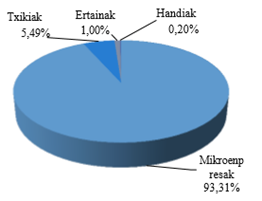
\includegraphics{enpresa_tamaina}
    \centering
    \par{Iturria: \citeauthor{confebask2014dimension} (\citeyear{confebask2014dimension})}
\end{center}

EAEko enpresen tamainari erreferentzia eginez, \ref{fig:enpresa_tamaina} irudian ikus daitekeen moduan, honako hauek dira \citeauthor{confebask2014dimension}-ek (\citeyear{confebask2014dimension}) eskainitako datuak: enpresen \%93,31 mikroenpresak dira eta 10 langile baino gutxiago dituzte; \%5,49 berriz enpresa txikiak dira, hau da, 50 langile baino gutxiago dituzte; \%1 enpresa ertainak dira, gehienez 250 langile dituztenak; eta soilik \%0,2 dira enpresa handiak, 250 langile baino gehiago dituztenak.

Nahiz eta EAEko enpresen kopuru handiena mikroenpresak izan, langileen kopuruaren banaketa enpresaren tamainaren oso bestelakoa da. Hona hemen \citeauthor{confebask2014dimension}ek (\citeyear{confebask2014dimension}) eskainitako datuak, enplegua enpresaren tamainaren arabera:

\begin{center}
    \captionof{figure}{\textit{EAEko langileen banaketa enpresa motako}}
    \label{fig:langile_banaketa}
    \centering
    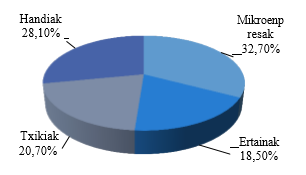
\includegraphics{langile_banaketa}
    \par{Iturria: \citeauthor{confebask2014dimension} (\citeyear{confebask2014dimension})}
\end{center}

\ref{fig:langile_banaketa} irudian ikus daitekeen moduan, mikroenpresek langileen \%32,7 soilik dute, nahiz eta enpresa kopuruaren \%93,31 izan. Enpresa txikien kasuan berriz, langileen \%20,7 enpresa mota hauetan egiten du lan eta ertainetan berriz, langileen \%18,5 aritzen da. Enpresa handien kasuan ordea, nahiz eta enpresa mota hauen kopurua oso murritza izan, langileen \%28,1 ari da bertan lanean.

Enpresa hauen bezeroak munduko herrialde ezberdinetan daude banatuta, enpresetako diru sarrera garrantzitsu bat kanpo merkatuetatik etorriz. Aldi berean, beste herrialde batzuetako produktu ugari ekartzen dira hona egunerokotasunean, esan bezala beste herrialde batzuekiko dependentzia handituz, Covid-19aren testuinguruan argi geratu den moduan. Datuetan sakonduz, \citeauthor{eustat2022kanpo}-en (\citeyear{eustat2022kanpo}) datuen arabera, EAEko ondasunen esportazioak 2619,3 milioi eurokoak izan dira eta inportazioak berriz, 2238,3 milioi eurokoak 2022ko martxoan. Iazko datuekin alderatuz, \%11ko eta \%31ko igoera nominala izan dute, hurrenez hurren.

Aipatutako informazio guztia aztertu ondoren, argi ikusten da aurretik deskribatutako globalizazioaren fenomenoa EAEn ere presente dagoela eta horren parte dela. Azken finean, bertako egoera ekonomiko, politiko, kultural eta soziala erabat baldintzatuta dago mundu mailan dauden joerekiko, nahiz eta tokian tokiko ohitura eta errealitateak pisu handia izan. Teknologia berrien eraginez, distantzia fisikoak desagertu diren heinean, munduko edozein eskualdetan gertatzen denak eragin zuzena eta berehalakoa izan dezake gure eguneroko bizitzan.

Hortaz gain, enpresetako jarduna merkatu berrietara zabaltzeko helburuarekin bertako enpresek nahiz atzerrikoek herrialde ezberdinetan filial eta ofizinak irekitzen dituzte. EAEn ere sektore ezberdinetako multinazional ugarik ireki dituzte egoitzak azkeneko hamarkadetan eta, horrez gain, hainbat proiektu jarri dira martxan instituzioetatik hauekin elkarlanean. Azken finean, globalizazio kontestu batean estrategia garrantzitsuenetako bat enpresen nazioartekotzea da, beren jatorrizko kokapenetatik kanpo dauden merkatuetara bideratzea, ulertuz modu hau dela modu konplexu eta interesgarriena enpresen hazkunde eta garapenerako (\cite{larrinaga2005internacionalizacion}).

Horren adibide dira Amazon, Microsoft eta Google bezalako multinazionalek EAErekiko erakutsi duten interesa eta beraien presentzia bertan handitzeko hartu duten konpromisoa. Amazonen kasuan esaterako Trapagaranen du egoitzetako bat eta Oiartzunen logistikako zentro baten eraikuntzaren proiektua alboratu ondoren, Arabako hainbat lursail aztertzen ari dira hazkunde esponentzialari erantzuteko. Hain zuzen ere, bost aldiz handitu du eta EAEko langile kopurua 2019tik (\cite{irigoyen2021amazon}).

Microsoft enpresa multinazionalaren kasuan berriz, Eusko Jaurlaritzarekin elkarlanean \textit{AI for Earth} proiektuan aritu dira, inteligentzia artifizialean oinarritzen diren proiektu berritzaileak bultzatzeko helburuarekin. Bertatik, bi proiektu jarri dira martxan. Lehena, turbina eoliko flotanteen konportamendua aztertzean datza, energia berriztagarriaren produkzioa maximizatzeko. Besteak berriz, 2018ko udan izan zen onddo defoliatzaileen erasoa hobeto ezagutzea du helburu, etorkizunean gerta daitezkeen egoera berdinei aurre egiteko (\cite{microsoft2020microsoft}).

Adibide hauen bitartez argi ikusten da multinazional hauek duten gaitasun ekonomiko eta zientifikoa arlo oso desberdinetan proiektu ezberdinak martxan jartzeko. Baina aldi berean enpresa hauek estuki baldintzatuta daude hezkuntza esparruan aurrera eramaten diren ikerketa proiektuekin. Horregatik, enpresa handien beharrek hezkuntzaren etorkizuneko norabidea asko baldintzatzen dute, beraien beharrak asebetetzera bidean. Hain zuzen ere, horren adibide garbia da EAEn Euskal Herriko Unibertsitatearen (EHU) \textit{Quantum Center} jarri dela martxan EHUko sei fakultate eta eskoletako 83 ikertzailerekin. Honen helburu nagusia adituak sortzea da enpresen beharrei erantzuteko, eskakizun handia baitago International Business Machines (IBM), Microsoft, Google eta Airbus bezalako multinazionaletatik besteak beste (\cite{gamez2020euskadi}).

\section{GAFAM}\label{sec:gafam}

Multinazional hauen ezaugarritzean sakonduz, sekulako inpaktua dute digitalizazio merkatua kontrolatu eta monopolizatzen duten enpresa teknologiko multinazional nagusiek, eta beraien artean bost erakunde bereizten dira: Google, Apple, Facebook, Amazon eta Microsoft. Bost erakunde hauei erreferentzia egiterakoan GAFAM ezizena erabiltzen da. 

Google, mundu mailan aurki daitekeen bilatzailerik arrakastatsuena da, erabiltzaile gehienek sarean informazio bilaketak egiteko erabiltzen dute orokorrean. Baina, plataforma honen helburuak, lehen puntu honetatik haratago doaz. Bere algoritmoari esker lortu daitekeen ikusgarritasuna kontuan hartuta, plataforma online gehienen muina da. Eskaintzen dituen zerbitzu desberdinak egunetik egunera hazten dira eta hauetako bakoitzak ezaugarri eta funtzionaltasun propioak ditu, erabiltzailearen beharrei modu erakargarri eta berritzaile baten erantzuten dienak.

Amazon, mundu mailan aurkitu daitekeen online denda esanguratsuena da, katalogo guztiz osatu bat eskaintzen diona erabiltzaileari. Kategoria desberdinetan, sektore eta prezio aniztasun handiak kontrolatzen ditu.

Facebook, mundu mailan erabiltzaile gehien konektatzen dituen sare soziala da. Hauen bitartez, pertsonak haien artean konektatzeaz gain, informazioa, eduki audiobisuala, notiziak eta bestelakoak partekatzen dituzte.

Apple, denetariko software eta gailu elektronikoak fabrikatu eta garatzen dituen enpresa multinazionala da. Haien produktu esanguratsuenen artean, \textit{iPod}, \textit{iPhone} eta \textit{iPad}-a daude eta softwareari dagokionez, Applek \textit{MacOS X} sistema operatiboa eta \textit{Safari} web nabigatzaileak garatu ditu.

Microsoft, mundu mailan aurkitu daitekeen software garatzaile garrantzitsuena da. Bere garapen handiena, munduan gehien erabiltzen den \textit{Windows} sistema operatiboa da. Hortaz gain, bere produktu arrakastatsuenen artean \textit{Office suite} ofimatika produktua dago.

GAFAM enpresek, teknologia neutrala eta beti positiboa den ideia transmititzen dute, eta mundua haien arauen arabera interpretatzen dugu. Balore burtsan lehenak dira, azken finean, irakurtzen, entzuten, ikusten dugun guztian interbentzio handia dute: nola lan egiten dugun, nola erosten dugun eta zelan erlazionatu eta dibertitzen garen, besteak beste. Hortaz gain, pandemian zehar hauen erabilera handitu denez, hazkunde mugagabea duten enpresak bihurtu dira (\cite{eavis2020big}).

\textit{Forbes} editorialaren arabera, GAFAM, munduko bost firma baliotsuenak dira. Estatistikak ez daude zuzenki erlazionatuta irabazten duten diruarekin, baina, hauen balioa, diru sarrera gehiago dituen enpresa batenak baino handiagoa da. Azken finean, enpresa mugagabeak, gobernu partiduak, Gobernuz Kanpoko Erakundeak (GKE) eta denetariko elkarteek, enpresa hauek barik bizirautea ezinezkoa da.

\begin{center}
    \captionof{figure}{\textit{GAFAM enpresen etekinen igoera 2019 eta 2020 artean}}
    \label{fig:gafam_etekinak}
    \centering
    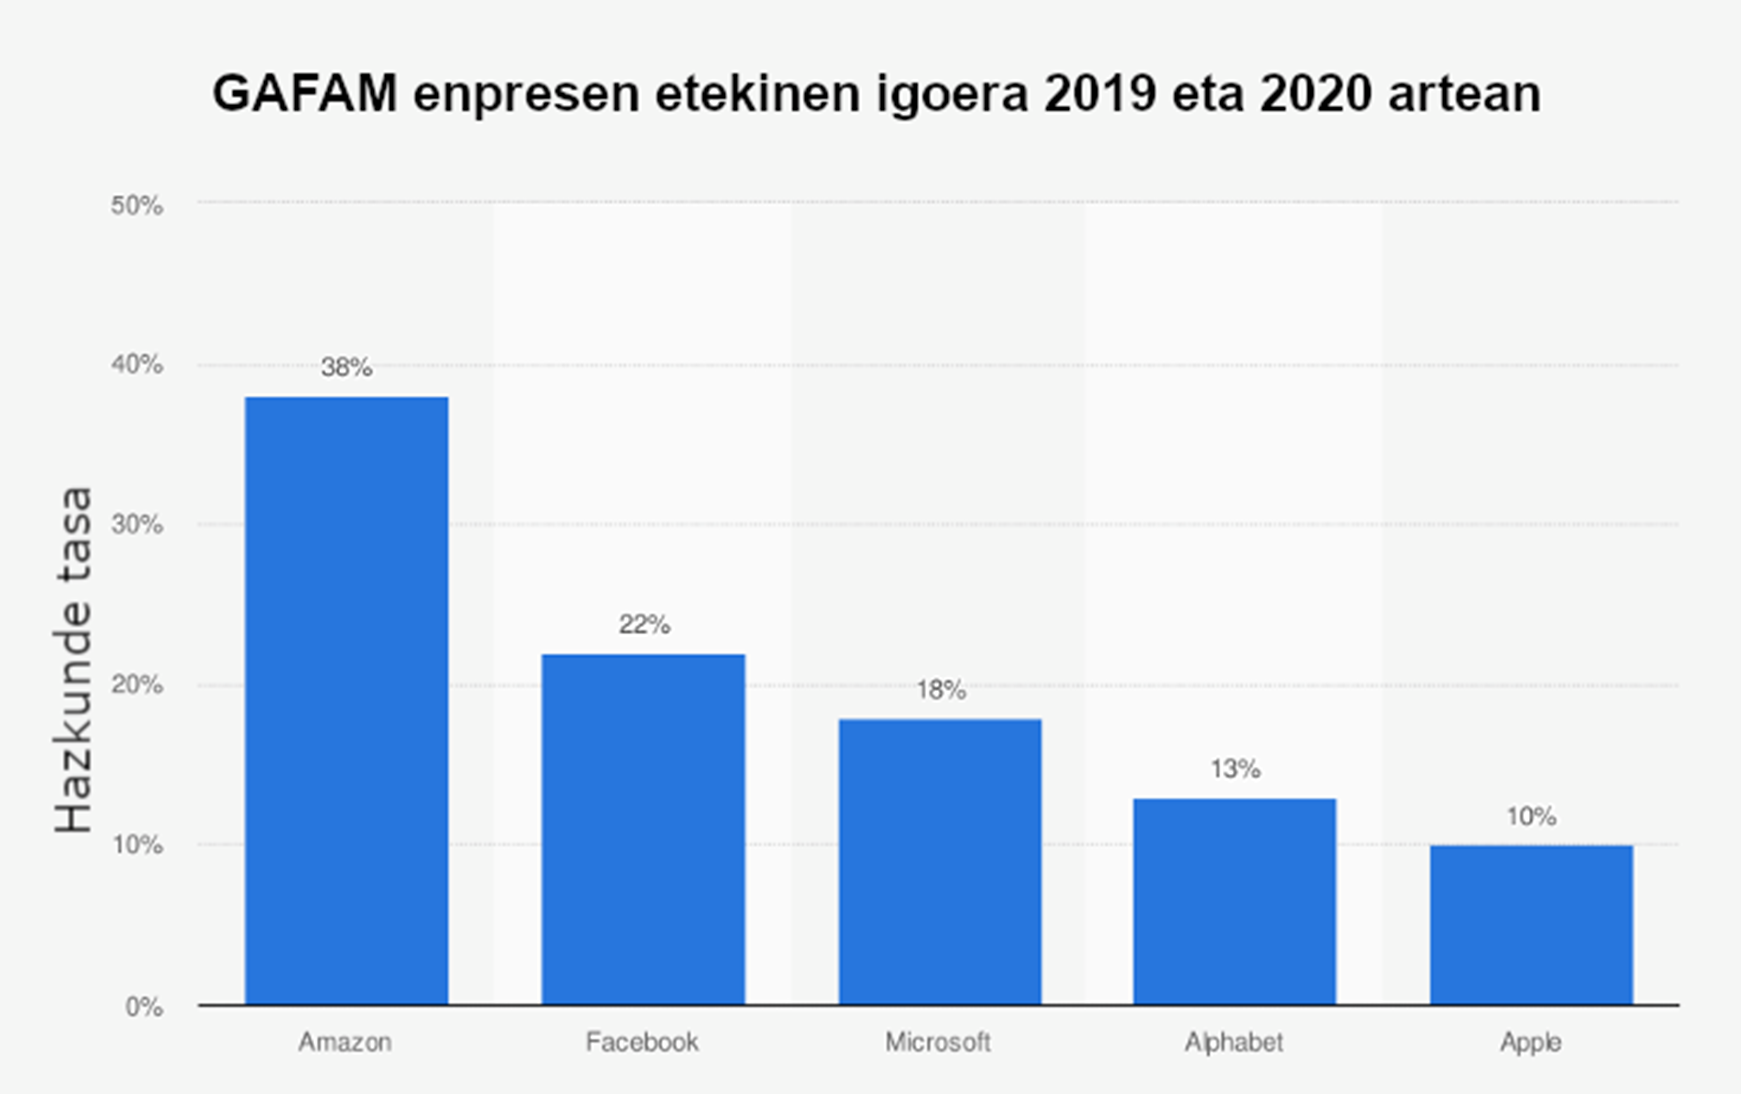
\includegraphics{gafam_etekinak}
    \par{Iturria: Sorkuntza propioa. Abiapuntua: \citeauthor{statista2021gafam} (\citeyear{statista2021gafam})}
\end{center}

Honen eredu argia, 2021 urtean bost enpresa hauek era bateratu batean izan duten irabaziak 259.000 milioi estatubatuar dolar zifra gainditu izana. \ref{fig:gafam_etekinak} irudian ikus daitekeen moduan, 2019 eta 2020 urteen artean GAFAM enpresak izan duten irabazien gorakada nabarmena da.

Monopolio bat mantentzea leporatzen zaie. GAFAM taldea bost enpresa desberdinek osatzen badute ere, ez dira haien arten konpetentzian dauden multinazionalak. Bakoitzak bere esparruan merkatu berriak garatzen lan egiten du eta haien artean sare indartsu eta aberatsa osatzen dute. \citeauthor{thiel2014competition}-ek (\citeyear{thiel2014competition}), PayPal plataformaren fundatzailetako bat, esandakoaren arabera:

\begin{adjustwidth}{3em}{0pt}
"Sare efektuak, produktua geroz eta pertsona gehiagok erabili, produktua erabilgarriagoa bihurtzen dute. Hortaz, erabiltzaile kopurua hain handia izanik, erreza da enpresa hauek sisteman haien arauak inposatzea."
\end{adjustwidth}

Honen inguruan, \citeauthor{de2019guia}-k (\citeyear{de2019guia}) hurrengoa adierazten du:

\begin{adjustwidth}{3em}{0pt}
"Enpresa hauen botereak estatua desafiatzen dute. Bankuen, botere finantzarioak adibidez estatuaren babesa behar duen bitartetan eta haien artean ulertzera behartuta dauden honetan, enpresa teknologikoek botere publikoen gaineko boterea jarduten dute."
\end{adjustwidth}

\section{GAFAM enpresak hezkuntzan zer?}\label{sec:gafam_hezkuntza}

Behin GAFAM enpresak ezaugarrituta, beharrezkoa da hauek hezkuntzaren esparruan eramaten duten jardunaren berri ematea. GAFAM enpresek hainbat helbururekin, nabarmenak edo ezkutukoak izan, haien ekosistema digitalak ikastetxeetan infiltratzeko asmoak argiak dira. Hezkuntzaren industriako erabiltzaileekin konektatu eta haien negozio ereduak, lotura emozionalak edota teknologiara hurbiltzeko forma ezberdinak ezartzea (\cite{herranz2018gafam}).

Hezkuntza mundura hurbildu eta geratzeko etorri dira enpresa hauek. Azken finean, erabiltzailearengan eragina duten ondorengo puntuak erakargarri egiten ditu bere baitan: eskolako bizitza eta bizitza erreala konektatzen dituzte, komunikatzeko eta erlazionatzeko erak aldatuz.

\begin{itemize}
    \item Erabiltzailea ezagutzen dute, izan ere, haien negozio ereduak honetan oinarritzen dituzte.
    \item Erabilera errutina berriak txertatu dituzte, erabiltzailearen esperientzia puntu garrantzitsuenetariko bat da enpresa hauentzat eta ikastetxeek eguneroko bizitzan kontestu desberdinetan hain presente dauden praktikak bereganatu ditu. 
    \item Lan egiteko era berriak, portaera berriak eta orokorrean ohitura aldaketak txertatu dira.
    \item Berrikuntza eta abangoardia hitzak presente daude, hezkuntza Google edo Apple izenekin erlazionatzen diren momentua eta zertifikatu hauek izatea erakargarria egiten dute.
\end{itemize}

Ikuspuntu soziologiko batetatik, generazio berriek positiboki baloratzen dute azkarra eta instantaneoa dena. Hezkuntzak eta ikastetxeak erritmo motelean eta era errepikakor batean aurrera egiten duten bitartean, \citeauthor{herranz2018gafam}ek (\citeyear{herranz2018gafam}), GAFAM enpresek sistema desafiatzen jarraitzen dutela dio proposamen erakargarri eta dinamikoagoekin.

Enpresa hauek, doakotasun faltsua eskaintzen dute ikastetxeetara hurbiltzerako orduan, haien zerbitzuak doan eskainiz, baina estrategia komertzialak besterik ez dira. Benetako asmoa, erabiltzailea ikastetxeko testuinguruan ezagutzea da, horrela hezkuntzaren beharrei erantzuteko negozioa garatzen dute negozio moduan. Hortaz gain, haien ekosisteman bereganatzen zaituzte, hardware, software, erreminta desberdinak, formakuntza eta zertifikatuekin, besteak beste. Honek, beste ekosistemekin konektatzea zailtzen du eta ez da erreza hemendik ateratzea.

Hezkuntza mundura hurbiltzeko asmoak argiak dira, azken finean enpresa hauen hazkunde eta garapenerako erabiltzaile baliotsuak dira. Ondorengo puntuetan enpresa hauen helburuen artean agerikoak direnak aipatzen ditu \citeauthor{herranz2018gafam}ek (\citeyear{herranz2018gafam}): Irabaziak lortzea: hezkuntza sektoreak, fakturazio eta irabazi hazkunde handiak eskaintzen dituen eremua da, aldi berean, negozio linea berriak garatzeko aukera ere.

\begin{itemize}
    \item Irakasle eta ikasleei laguntzea eguneroko lan eta jardueretan.
    \item Erabiltzaile datuak eta datu pertsonalak eskuratzea haien produktuen garapenerako.
    \item Filantropia erabiltzen dute askotan, helburu komertzial oso argiak definituta dituztelarik.
    \item Bezeroak fidelizatzea hauek umeak direnetik. Produktuen bitartez behar berriak sortzen dituzte ikaslearengan, bai eskolako eta bai etxeko esparruetan.
    \item Programazio eta konputazio trebetasunak garatzea ikasleengan, etorkizunean haien langile bihurtu daitezkeen erabiltzailean.
\end{itemize}

Baina, GAFAM enpresek badute hain agerikoak ez diren asmoak eta hezkuntza munduarekin zuzenean kontraesan handiak dituena, \citeauthor{herranz2018gafam}ek (\citeyear{herranz2018gafam}) ondorengo puntuetan deskribatzen dituenak, adibidez:

\begin{itemize}
    \item Enpresa hauek haien estandarrak hezkuntza munduan inposatzen saiatzen ari dira. Irakaskuntzaren praktikan eragina duten formakuntza saioak, doakotasun estrategiak eta zertifikatuak txertatuz.
    \item Hezkuntza zentroetan eta ikaslearen eta irakaslearen bizitzetan algoritmo eta inteligentzia artifizial estrategia masiboak txertatzen dituzte, ikasketa pertsonifikatuaren azken formula izatearen lemarekin.
    \item Datu pertsonalak zertarako erabiltzen dituzten zalantza handia dago oraindik, horien artean: adingabea babesten dute? Zer egiten da haien gailuekin grabatzen den material audiobisual guztiarekin?
\end{itemize}

Filantropiaren ideia faltsua hezkuntzaren bitartez erabiltzen da, non aberatsek eta hauen fundazio "filantropikoak", ez daude donazioen eta laguntzen atzean jada. Aberatsek zuzendu eta bideratzera pasatu dira, non gobernuak, enpresak eta GKEak era bateratu batean lan egiten duten, hezkuntzaren merkatuan dauden hazkunde aukerei heltzeko, politika berriak diseinatuz; edo GAFAM enpresen hedapena "konponbide teknologikoa" eskainiz, hezkuntzaren salbazio eta modernizazio eran apainduta digitalizazioaren bitartez. Baina atzean, XXI. mendeko urrezko negozio ideia dakarrena: etorkizuneko erabiltzaile eta kontsumitzaile generazio oso baten datuak. Hezkuntza eremura adimen artifiziala (\textit{artificial intelligence}, AI), \textit{Big Data}, gauzen interneta (\textit{Internet of Things}, IoT), blokeen katea (edo \textit{blockchain}) edota hodei-konputazioa (\textit{cloud computing}) aplikatuz (\cite{diez2022invasion}).

Posible al da justizia sozialerako bidean lan egiten duten ikastetxeek, software eta hardware produzitzaile multinazionalen instrumentuen erabilera masibo bat egitea? Horregatik, irakasleek, digitalizazio prozesu hauek beraien lanean duten inpaktuaren inguruan pentsatzeko beharra dugu nahitaez. Hausnarketa pedagogiko minimo batek, azalera eramaten du nola plataforma birtual hauek instalatzen duten dinamika berriek gure lan egiteko modua hautatzeko aukerak moztu eta deuseztatzen duten. Hortaz, dialogo aukerak geroz eta txikiagoak diren momentuetan, kritikoa eta elkarrizketarako irekia espiritua nola sortu daitekeen inguruan hausnartu behar da. Edo, lan egiteko eraren kontrola nola berreskuratu behar den, aurretik software diseinatzaileen eskutatik moldeatuta badatoz (\cite{almazan2020covid}).

\section{GAFAM enpresak EAEko hezkuntza sisteman}\label{sec:gafam_eae_hezkuntza}

Laburbilduz, azken hamarkadetan teknologiak eman duen garapen izugarri baten kontestuan eta digitalizazio prozesu etengabe batean aurkitzen da gizartea. Honek guztiak, erabiltzailearentzat bere datuen gaineko kontrolaren erabateko galera suposatu du. Aldi berean, enpresa handi gutxi batzuen esku geratuz informazio guztia, irabaziak lortzeko bitarteko bihurtuz (\cite{decode2017what}). Egoera honetan, datu kantitate horiek ez dira erabilgarriak onura publikorako zerbitzu eta irtenbideak sortzeko. Kontrara, honek desberdintasun ekonomikoak eta eraginkortasun eza ekartzen ditu.

EAEren kasuan ere, ikus daiteke hezkuntzaren digitalizazioaren bidean Eusko Jaurlaritzak hartu duen norabidea eta aldi berean, horri aurre egiten dioten proposamenen garapena. 2022eko apirilean, Eusko Jaurlaritzak Google, teknologia digitalen enpresa multinazional pribatuaren tresnak ikastetxe publikoetan erabiltzeko, gutxienez lau urterako hitzarmena sinatu zuen. Hezkuntza Saileko ikastetxeetan \textit{Google Workspace for Education} zerbitzuak erabiltzeko hitzarmena sinatzen dute \textit{Google Cloud Emea Limtied} enpresak eta Eusko Jaurlaritzak eta bi aldeek hainbat konpromiso hartu dituzte. Horrela dio \citeauthor{apaolaza2022google}-k (\citeyear{apaolaza2022google}):

\begin{adjustwidth}{3em}{0pt}
“Hezkuntza Sailak Googlen zerbitzuak ezartzeko faseak definituko ditu eta zerbitzu horietarako sarbideak erraztuko dizkie irakasle zein ikasleei, baita beharrezko “prestakuntza-planak” egin ere. Gainera, Googlekin “lankidetzan” aritzeko konpromisoa hartu du Hezkuntza Sailak; talde misto bat sortuko dute horretarako, eta “tresna berriak probatzeko” \textit{betatester} talde bat ere sortuko dute ikasleen artean, ikastetxeetan Googlen zerbitzuen erabilera sustatzeaz gain.”
\end{adjustwidth}

\citeauthor{ej2022aldizkari}-ren (\citeyear{ej2022aldizkari}) aldizkariak jasotzen duen hitzarmenak, bai Eusko Jaurlaritzak eta bai Googlek sinatutako baldintzak irakurri daitezke. \citeauthor{apaolaza2022google}ren (\citeyear{apaolaza2022google}) hitzetan oinarrituz, aldizkariak arrazoi ekonomikoak ez ditu inondik inora azaltzen. Gainera, Google enpresa bat izanez, etekina aterako duela jakina da, baina hau ere ez da adierazten. Gazteen erabilerarekin lortutako datu pertsonalen tratamendua eta erabileran oinarrituko dela ondorioztatu daiteke. Erabaki honen bitartez, Eusko Jaurlaritzak Hezkuntza Sailaren menpeko ikastetxeetako ikasleen datuak pribatizatzearen alde egin du.

Googlerekin sinatutako azken hitzarmen honetaz gain, Eusko Jaurlaritzak harreman historikoa du Microsoftekin eta eskoletako digitalizazioa enpresa honen esku utzi du. \citeauthor{barcenilla2021gv}-k (\citeyear{barcenilla2021gv}) jasotzen duen moduan, “EAEko eskola publikoetan ikasleek erabiltzen dituzten plataforma digitalak Microsoftekin hitzartu ditu Eusko Jaurlaritzak, bost urtean multinazionalera 3 milioi euro bideratuz”. Sare publikoa osatzen duten EAEko ikasleen \%51 Microsoften datu-basean daude. 

Enpresa multinazional hauek hezkuntza sistemaren barruan daude jada eta Google eta Microsoft enpresek sortutako erremintak eta aplikazioak Euskal Herriko ikastetxe pribatu eta publiko ia guztietan erabiltzen dira.

Erabaki honen aurrean kritiko diren norbanako eta eragileak azaltzen dute software itxi hauek, hezkuntza sistemaren barruan sarbidea izateak, ikasle adingabeen datuak eta hauen eskubide urraketan eragin larria duela. Doakotasun faltsua eskaintzen dute eta trukean datu pertsonalak eskuratzen dituzte. \citeauthor{hl2019komunikatua} \citeyear{hl2019komunikatua} taldearen ustez, enpresa pribatuek egin dute digitalizazioaren gidaritza orain arte, eta planik ez dago Eusko Jaurlaritzako Hezkuntza Sailean. Horrela bada, hezkuntza eredu burujabeago batera bultzatzeko nahian mugimendu ezberdinak sortu behar dira, zentroetan software libreak inplementatuz, adibidez.

\section{Burujabetza digitala eta hezkuntza librezalea}\label{sec:burdig}

Kontestu honetan egitasmo ezberdinak sortu dira aipatutako egoera honi buelta eman asmoz, erronka digitala XXI. mendeko erronka nagusi moduan hartuz. Aipatzekoa da \citeauthor{ehd2021manifestua}k (\citeyear{ehd2021manifestua}) argitaratutako manifestua, teknologia jendartearen zerbitzura jartzeko helburuarekin. Hauen esanetan, auzi honek 4 esparrutan eragin du gutxienez: Demokraziaren esparruan, lanean, hezkuntzan era gizakian berarengan. 

Hezkuntzaren esparruan duen eraginak kezkatuta, Euskal Herrian alternatibak planteatzera bidean, 2017an Hezkuntzan ere Librezale taldea jarri zen martxan, irakasle, ikasle, guraso eta eragileez osatua. Hainbat puntuz osatutako komunikatu bat dute kaleratua eta zenbait material eskuragarri dute euskal hezkuntzan ematen den egoeraren aurrean alternatiba digital libreen erabilera bultzatzeko (\cite{hl2019komunikatua}). Hainbat kezka mahaigaineratzen dituzte:

\begin{itemize}
    \item Ikasleen datuak enpresa pribatuen esku uzteak beraien pribatutasuna galarazten du, ikaslea produktu bihurtuz. 
    \item Chromebook bezalako gailuetan inbertsioak egitea arduragabekeria da, 5 urteren buruan zaharkituak geratzen direlako, berrerabilpena galaraziz.
    \item Gailu digitaletan euskararen presentzia enpresa pribatuen agindu eta nahietara uztea euskararen aurkako neurria da. Konkretuki, Chromebooketako hainbat atal ez daude euskaraz gaur egun. 
    \item Ikasleei tresna digital berdinak erabiltzera mugatzea, hezkuntza digitala murriztea da.
    \item Hezkuntza komunitatean tresna hauekiko dependentzia sortzea arazo larria da. Instituzioetatik enpresa pribatuen erabiltzaile eta bezeroak sortzen ari dira. 
\end{itemize}

Honen aurrean, ikasleen eskubide digitalak eta pribatutasuna errespetatuz eta bitarteko teknologiko auditagarri, berrerabilgarri, libre eta gardenak erabiliz, digitalizazio etiko, arduratsu, eraginkor eta euskalduna bermatzeko aukerak sortu behar dira (\cite{hl2019komunikatua}). 

Hori epe luzerako begiradarekin diseinatu behar da gure hezkuntza sistema bere burua eraldatzen joan dadin, baita digitalizazioan ere. Digitalizazioak hezkuntzari aukera askotarikoak eskaintzen dizkio, beti ere, ikaslearen ahalduntzearekin zuzenean lotuak. Ahalduntze horrek, gaitasun digitalak garatzeaz haratago, menpekotasunak sortzea saihestu eta ikasleak ingurune digitalean boterea hartzea eskatzen du, herritar digital burujabeak izan daitezen (\cite{hl2019komunikatua}).

Bide honetan, ikastetxeko datuak multinazional handien esku uzteari aurre eginez, software libreen erabileraren alde pausuak eman dituzte hainbat ikastetxetan. Tolosako Lanbide Heziketako zentroan 3 produktu nagusi dituzte martxan: Postarako \textit{Zimbra}, klaseak kudeatzeko \textit{Moodle} eta \textit{NextCloud} informazioa artxibatzeko hodei moduan (\cite{garcia2020}). Beste adibideetako berriz, Elgoibarko Fabrikazio Aurreratuaren era Digitalaren Campusa izango litzateke. 

Euskal Herrian eman diren adibide hauez gain, estatuko beste hainbat lekutan, nahiz, Europa mailan hainbat egitasmo jarri dira martxan. Esaterako, Katalunian \textit{Xnet} eskubide digitalen plataformak aurkeztu duen \textit{Digital Democràtic} suitea. Honek, ikastetxe eta hezkuntza esparruari erreminta digital ugari eskaintzen dizkie, software libre eta auditagarria bat esaterako. Honen asmoa Google \textit{Meets}, \textit{Drive} edo \textit{Calendar} bezalako tresnak ordezkatzea. Plataforma hau, Google bezalako multinazionalen aurrean alternatibarik ez zegoelako jaiotzen da 2018 urtean (\cite{vicente2022}). Horrez gain, Valentziako erkidegoa da ikasleen pribatutasuna babesteko kode irekiko tresnak diseinatu dituen Europar Batasuneko eskualde bakarra (\cite{barcenilla2021gv}).

Bukatzeko, beste adibideetako bat \citeauthor{decode2017what} \citeyear{decode2017what} proiektu esperimentala da, zeinak, helburu moduan alternatiba praktikoak sortzea duen, pertsonen datuak babestu eta burujabetza digitala bultzatzeko. Hau Europa mailan landutako saiakera da. 
\chapter{Marko teorikoa}\label{cha:markoa}
Lan hau kokatzen den marko teorikoa aztertzen hasteko garrantzitsua da hezkuntza teknologikoak egungo hezkuntza sisteman duen rola ulertzea. Horretarako, zer den teknologia jakin behar da lehenik eta behin. Teknologia, \citeauthor{harluxet2019awareness}-k (\citeyear{harluxet2019awareness}, 2. definizioa) egindako definizio entziklopedikoan oinarrituz, gizakiak erabiltzen dituen tresna, makina, prozedura eta metodo teknikoen multzoa. Definizioa kontuan izanda, hezkuntza bera teknologia bat dela ondorioztatu daiteke.

\section{Hezkuntza teknologikoa}\label{sec:heztek}

Hausnarketarekin aurrera jarraituz, bi galdera formulatu daitezke. Lehena, zein da hezkuntzak duen funtzioa gure gizartean? Bigarrena, eta esaldi korapilatsu bat sortuz: hezkuntza teknologia bat izanda, zertarako irakasten da hezkuntza teknologikoa?

Hezkuntzak gizartean duen funtzioaz hitz egiterakoan, gazteria etorkizunerako prestatzea dela esan daiteke. Teknologia bat izanik, prozesu multzo bat da, ikasle bat ume izatetik heldu izan arte igarotzen dena, jakintzak eskuratzen joateko. \citeauthor{tarabini2020que}-k (\citeyear{tarabini2020que}) aipatzen duen bezala, historian zehar, gizarte kapitalista agertu zenetik, korronte desberdinek ondorio berdina izan dute: hezkuntzaren funtzioak bi dira, pertsona lan munduan integratzeko prestatzea eta gizartean integra daitekeen pertsona identitatea sortzea. Beraz, teknologia honen funtzioa zehaztuz, jakintza, ezagutza eta trebakuntzaren transmisioa dela esan daiteke, aurrez aipatu diren bi helburuak lortzeko.

Puntu honetara iritsita, pentsa daiteke hezkuntza teknologikoaz hitz egiten denean, gizartearen historian garatu diren prozesu teknologikoen inguruko ezagutza transmititzeaz hitz egiten dela. Baina hau ez da horrela. \citeauthor{tarabini2020que}ren (\citeyear{tarabini2020que}) testuan irakur daitekeen moduan, sistema kapitalistaren menpe dago hezkuntza, eta XX. mende amaieratik iraultza teknologiko etengabean dagoen sistema da hau (\citeauthor{del2016industria}, \citeyear{del2016industria}; \citeauthor{ghobakhloo2020industry}, \citeyear{ghobakhloo2020industry}). Beraz, kapitalismoaren beharrei erreparatuz, ezin da finkatu hezkuntza teknologikoaren helburua zein izango den datorren urteak ikasten igaroko dituen ikasle batentzat: iraultza aurrera doan heinean, lan mundura integratzeko behar dituen trebetasunak aldatuz joan daitezke, eta zentzugabekeria da uneko trebetasunen jakintza garatzea, urteak aurrera egin ahala zaharkituak geratu daitezke eta. Horregatik, eta \citeauthor{sole2020cambio}-k (\citeyear{sole2020cambio}) aipatzen duen moduan, hezkuntza sistemaren joera konpetentzien garapenera doa. Baina konpetentziekin hasi baino lehen, XXI. mendeko gizartea ulertu behar da.

\subsection{XXI. mendeko gizartearen erronkak}\label{subsec:xxi_erronkak}

Gaur egungo gizarte mailako erronka orokorrak definitu eta horiei aurre egiteko, 2000-2015 milurteko garapeneko helburuak berreskuratuz, 2015eko irailaren 25ean Agenda 2030 onartua izan zen Nazio Batuen asanblada orokorrean. Bertan, Garapen Iraunkorreko Helburuak (GIH) zehazten dira, zeinak politika publikoak hobetu eta lehentasunak definitzeko kontestu bat finkatzen duen lurralde bakoitzeko errealitatea kontuan edukiz (\citeauthor{vasco2017contribucion}, \citeyear{vasco2017contribucion}).

Agenda honen barruan zehazten diren edukietan sakonduz, garapen iraunkorrerako 17 helburu zehazten dira. Helburu hauek, ekintzarako dei unibertsal bat dira pobreziarekin amaitzeko, planeta babesteko eta mundu osoko pertsonen bizitza eta aukerak hobetzeko (\citeauthor{nbe2021}, \citeyear{nbe2021}). Hauek guztiak, planetarentzat eta gizartearentzat orokorrean garrantzia berezia duten 5 esfera landuz burutu nahi dira.

\begin{itemize}
    \item Pertsonak: pobrezia eta gosea amaitzea bere forma eta dimentsio guztietan, eta pertsona guztiek beraien ahalmenak duintasunez, berdintasunean oinarrituta eta ingurune osasuntsu batean bete dezaketela bermatzea.
    \item Planeta: degradaziotik babestea kontsumo eta ekoizpen jasangarrien, baliabide naturalen kudeaketa jasangarriaren eta aldaketa klimatikoari aurre egiteko neurri zehatzen bidez. Modu honetan, gaur egungo eta etorkizuneko belaunaldien beharrei erantzunez.
    \item Bakea: indarkeria eta beldurrik gabeko gizarte baketsu, justu eta inklusiboak sustatzea.
    \item Oparotasuna: pertsona guztiek bizitza oparo bat izan dezatela ziurtatzea eta garapen ekonomiko, sozial eta teknologikoa naturarekin bat etorriko dela ziurtatzea.
    \item Lankidetza: agenda ezartzeko beharrezkoak diren bitartekoak martxan jartzea mundu mailako aliantza baten bitartez garapen iraunkorra inplementatzeko. Guzti hau, mundu mailako elkartasun handiago batean oinarrituta eta bereziki pobreenen eta ahulenen beharretan arreta jarriz. Baina hau herrialde guztietako eragile eta pertsonen lankidetzarekin gauzatuta.
\end{itemize}

EAEn hau guztia lurreratzeko, I. Agenda Euskadi Basque Country 2030 dago, zeina 17 helbururen inguruan egituratzen den. Helburu hauek, herrialdeko 15 helburuei lotuta daude eta guztira 100 meta definitzen dira (\citeauthor{vasco2017contribucion}, \citeyear{vasco2017contribucion}).

Hezkuntza komunitateak ere aipaturiko norabidea elikatzeko konpromisoak hartuak ditu. Horren adibide da, Eskola Agenda 2030 programaren existentzia eta sortu zenetik, bataz beste, urtero 450 ikastetxe (publiko, itunpeko zein pribatu), 200.000 ikasle baino gehiago eta 15.000 irakaslek bertan parte hartu izana (\citeauthor{dv2021}, \citeyear{dv2021}). Horrez gain, aurrerago zehaztuko den moduan, hezkuntza teknologikoaren helburua eta dinamika bera, erabat bideratuta daude gizarte moduan ditugun erronka eta beharrei erantzun egoki bat ematera. Beraz, ezinbestekoa da lehenik eta behin egungo egoeraren analisi kritiko bat egitea eta jarraian, horiei erantzungo dieten planteamenduak garatzea. 

Erronka hauen baitan, hezkuntza mugimendu bat du da azken urteetan. Arazo garaikideei aurre egiteko hezkuntza digitalean burujabetza eta pentsamendu kritikoa nabarmentzea nahi dituena.

\subsection{Zientzia, Teknologia eta Gizartea}\label{subsec:ztg}

Alde batetik, gaur egungo gizartea etengabeko berrikuntza eta aldaketek ezaugarritzen dute. Hori dela eta, baliabide materialen (azpiegitura, makinak) beharrezkotasuna bigarren planoa batean geratzen da, geldiezinak diren berrikuntzen ondorioz azkar batean zaharkituta geratzen direlako. Kontestu honetan, baliotsuena norbanakoek sormenez, arduraz eta kritikoki ezagutzak sortu, elkarbanatu eta aplikatzeko duten gaitasunak dira (\citeauthor{acevedo1998ciencia}, \citeyear{acevedo1998ciencia}). 

Beste alde batetik, ezin uka daiteke teknologiak hartu duen garrantzia bizitzako alor guztietan eta hori dela eta, honen aldeko, kontrako edo erdi bideko posizioak hartuz joan dira hainbat esparru, \citeauthor{acevedo1998ciencia}ren (\citeyear{acevedo1998ciencia}) testuan irakurri daitekeen bezala. Teknologiarekiko jarrera ezberdin hauen arrazoi nagusia honek gizartean izan duen eraginean datza.

Nahiz eta teknologiak hainbat hobekuntza nabarmen ekarri herritarrei, honek aberatsen eta pobreen arteko arrakala handitzea ekarri du. Hau da, herrialde, lurralde eta talde sozial aberatsak geroz eta aberatsago izatea eta pobreak geroz eta pobreago izatea, nahiz eta, hasiera batean kontrakoa uste zen (\citeauthor{osorio2002educacion}, \citeyear{osorio2002educacion}).

Horren adibide da, Munduko Bankuaren datuen arabera, 2012an 896 milioi pertsonak eguneko 1,9\$ baino gutxiagorekin biziraun izana (\citeauthor{migoyaxxi}, \citeyear{migoyaxxi}). \citeauthor{menendez2017europe}-k (\citeyear{menendez2017europe}) egindako txostenak adierazten du pobrezia profil berri bat sortu dela. Pobrezian bizi diren pertsona hauek lan egiten duten (lanaldi partzialak, aldi baterako kontratuak edo lan autonomoak) baina aldi berean pobreak dira. Gaur egun, Europako langileen \%10ek osatzen dute profil hau.

Kontestu konplexu honetan, zientzia eta teknologiak soilik paper bat jotzen du gaur egungo joko zelaian eta jakinekoa da teknologia eta zientziak beste orientazio sentikorrago bat hartzen ez badute, aipatutako egoerak okertzen lagunduko dutela soilik dio \citeauthor{osorio2002educacion}k (\citeyear{osorio2002educacion}). Hori dela eta, ezinbestekoa da hezkuntza aktore klabe moduan hartuz, bertatik zer egin daitekeen aztertu eta garatzea.

Hezkuntzak funtzio sozial garrantzitsuak betetzen ditu. Tartean, berriz ere \citeauthor{acevedo1998ciencia}ren (\citeyear{acevedo1998ciencia}) hitzez baliatuz, belaunaldi berriei gizarte produktibo batean behar bezala funtzionatzeko gaitasun ezberdinak eskaintzea, nahiz eta etengabeko aldaketen ondorioz, hezkuntzaren funtzioa gizarteko partaide guztiengana luzatu, bizi osorako ikaskuntza ardatz hartuz.

Orain arte aipatu moduan, teknologia eta zientziak bizitzako esparru guztietan duen garrantziagatik eta belaunaldi berriak etorkizuneko erronkei aurre egiteko prest egoteko, hezkuntza teknologiakoren beharra ezinbestekoa da.

Hezkuntza teknologikoa, teknikak ulertu, hautatu, erabili, egokitu, ebaluatu eta sortzeko eta, azken finean, teknologiak ekoizteko aukera ematen dion prestakuntza da. Hau da, bakoitzaren ingurune teknologikoa modu naturalean arakatzen laguntzea eta kontsumitzaile kritiko eta erabiltzaile adimenduna izatea (\citeauthor{grau2016educacion}, \citeyear{grau2016educacion}).

Honen bitartez, hezkuntza ingurune teknologiko eta zientifikora zabaltzeko aukera eskaintzen da, horren gainean modu arrazionalean jarduteko. Horrez gain, ezagutzak batu eta horiek prozesu didaktiko bakarrean biltzea eta aldi berean, lanerako eta goi mailako ikasketetarako prestatzea. Azkenik, \citeauthor{grau2016educacion}k (\citeyear{grau2016educacion}) dioen moduan, ikasleen orientazio profesionalaren lagungarri izateko aukera ere ematen du.

Laburbilduz, hezkuntza teknologikoaren kontzeptua globala da eta inplikazio gradu, maila eta modalitate ezberdinak inplikatzen ditu, zeren eta bere helburua ez da ikaslea teknologikoa edo teknologian espezializatua izatea. Azken finean, hezkuntza teknologikoaren bidez balioetan oinarritutako hezkuntza txertatzea da xedea, hau da, teknologiak baloratzeko eta hauen ondorioak ebaluatzeko heztea, teknologien ebaluazioan publikoaren parte- hartzea ahalbidetzeko ezinbestekoa dena (\citeauthor{martin2000acercando}, \citeyear{martin2000acercando}).

Kontestu honetan, garrantzitsua da teknologiaren erabilera sustatzea ikuspegi humanista, kritiko eta arduratsu batetik, ikasleek ezagutzak sortu, ideiak transmititu, irtenbideak identifikatu eta produktu zehatzak garatzeko norberaren interesen arabera (\citeauthor{leal2019}, \citeyear{leal2019}).

Nahiz eta teknologia oso presente eduki egunerokotasunean, sarritan honen ikaskuntza termino abstraktuetan geratzen da. Horregatik, ikasleak teknologiaren baliagarritasunaz ohartarazteko garrantzitsua da hainbat gako kontuan edukitzea.

Alde batetik, teknologia proiektuak garatzeko erreminta bezala ulertzea. Hau da, ikasleen eskura egongo den erreminta bezala ulertzea teknologia eta ez alderantziz. Horretarako, \citeauthor{leal2019}en (\citeyear{leal2019}) ustetan, interesgarria ikusten da lantzen ari diren materiak teknologiako proiektu espezifikoekin lotzea. Beste alde batetik, garrantzitsua da tresna digitalen erabilera beste ikasgai batzuetara zabaltzea, beste ikasgai horien ikaskuntza bultzatu eta errazteko. Horretarako, beharrezkoa da alde batetik irakasleen mesedetara baliabide digitalak jartzea baina bereziki irakasleek ikasleak kontzientziatzea baliabide hauen erabilerak beraien ikaskuntza prozesua hobetuko duela.

Horrez gain, teknologiak sormena garatzeko, konponbideak sortzeko eta arazoak konpontzeko gaitasuna du. Horregatik, ikasleek beraien ikaskuntza prozesuak sinplifikatzeko, irtenbide sortzaileak sortzeko, proposamenak egiteko eta ideiak adierazteko teknologia bultzatu nahi da.

\citeauthor{leal2019}en (\citeyear{leal2019}) teoriarekin jarraituz, zientzia eta teknologiak aldaketa sakonak eragin dituzte alor sozial, ekonomiko, teknologiko eta mediatikoan. Horregatik, ikasleek horrekiko ikuspuntu kritiko bat garatzea garrantzitsua ikusten da hezkuntzako idealen parte delako eta aldi berean, ikasleek proposamenak egiteko erabiltzea ikuspegi humanista bultzatu eta aldaketa soziala bultzatuz.

Honetaz guztiaz gain, teknologiaren erabilera seguru eta arduratsua irakastea ikasleei. Elkarrekintzarako forma berriak erabiltzen diren momentutik, arrisku eta gatazka etiko berriei aurre egin behar zaie. Horregatik, garrantzitsua da teknologiaren erabilera arduratsu eta etiko bat bultzatzea. 

Hezkuntzako hainbat sektoretatik, ikasleei informazio eta ezagutza baino, eguneroko bizitzari aurre egiteko gaitasunak emateko beharraz ari dira. Horien artean egongo lirateke, talde lanarekin, komunikaziorako trebetasunekin, arazoen ebazpenarekin eta erabakiak hartzearekin lotutakoak. Horrez gain, mundu ikuskera zientifiko eta teknologiko bat duten ikasleak trebatzea espero du \citeauthor{acevedo1998ciencia}k (\citeyear{acevedo1998ciencia}). Aldi berean, hezkuntza teknologikoaren kontzepziotik, honek aukera handiak eskaintzen ditu konpetentzietara, disziplinartekotasunera, ikasleen motibaziora, gaien egokitasunera hurbiltzeko.

Orain arte aipatutako aspektu eta ezaugarri guztiak kontuan hartu eta bide horretan ekarpena egiten du Zientzia, Teknologia eta Gizartea (ZTG siglekin adierazia) mugimenduak.

Termino honek barne- biltzen dituen hiru aspektu nagusietan sakonduz, jakitun gara zientzien eta teknologiaren arteko bereizketa kritiko bihurtu dela, lehena alderdi askotan bigarrenaren zerbitzura dagoelako. Zentzu horretan, “tekno- zientzia” terminoak zientzia eta teknologiaren arteko hurbilpen bat gauzatzen du, politika, ekonomia eta ingurugiroarekin batera. Aldi berean, ZTG mugimenduak, zientzia eta teknologiaren garapena ingurune sozial eta politiko batean kokatzen ditu (\citeauthor{osorio2002educacion}, \citeyear{osorio2002educacion}).

Mugimendu honen helburua herritarren alfabetatze zientifiko eta teknologikoa sustatzea da, erabakiak hartzeko prozesu demokratikoetan eta zientzia eta teknologiarekin lotutako arazoen ebazpenetan parte har dezaten (\citeauthor{membiela1997revision}, \citeyear{membiela1997revision}).

Aipatutako lan egiteko proposamen hau zehaztuz, \citeauthor{hickman1987science}-ek (\citeyear{hickman1987science}) kontuan eduki behareko bost kriterio nagusi zehazten zituzten ZTG- ko edukietan:

\begin{itemize}
    \item Ea zuzenean aplikatu daitezkeen lantzen diren edukiak ikasleen eguneroko bizitzetan.
    \item Ea edukiak egokiak diren ikasleen garapen kognitibo eta heldutasun sozial mailarako.
    \item Lantzen ari den gaia gaur egun munduan ikasleentzat eta aldi berean helduentzat garrantzitsua ote den.
    \item Ezagutza horiek eskolaz kanpoko testuinguruetan aplikatu daitezkeen.
    \item Ikasleek interesa, ilusioa eta lanerako gogoa erakusten duten gaia ote den.
\end{itemize}

ZTGekiko lotura duten arazo sozialen arabera, 2 perspektiba nagusi definitzen ditu \citeauthor{rosenthal1989two}-ek (\citeyear{rosenthal1989two}). Alde batetik, komunitate zientifikotik kanpoko gizarte- gaiak, hala nola, berotze globala, gerra kimikoa edo elikagaietako pestizidak. Bestetik, komunitate zientifikoaren barneko gizarte- gaiak, zientziaren gizarte- ikasketa moduan deitzen direnak, non zientzia bera den gizarte- zientzien aztergai bere ondorio filosofiko, soziologiko, historiko, politiko, ekonomiko eta kulturalak jorratuz.

Mugimendu honen printzipioak eta edukiek izan beharreko ezaugarriak definitu ondoren, hau guztia ikasgelara nola lurreratu zehaztea beharrezkoa da. Nahiz eta unibertsitate eta bigarren hezkuntzako eremuetan garatu den mugimendu honen jarduna (\citeauthor{membiela1997revision}, \citeyear{membiela1997revision}), bigarren hezkuntzan ZTG markoaren printzipioak nola lurreratzen diren lantzen da. Horretarako hiru modu edo bide nagusi daude.

Horietako bat, ZTG txertoak izango litzateke. Ikasleak zientziaren eta teknologiaren ondorioez jabetzera bultzatzen dituzten alderdiekin lotutako arazoetarako tresna garrantzitsua bihurtzen dira (\citeauthor{osorio2002educacion}, \citeyear{osorio2002educacion}). 

Konkretuki, zientzia ikasgai bati ZTG alorreko gehikuntza bat egitean datza, beti ere zientziaren izaera eta teknologiarekin eta gizartearekin dituen inplikazioak berrikusi beharko lituzkeena. Baita ere aldi berean, herritarrek duten papera garapen tekno- zientifikoaren inguruko erabakietan.

Teknologiako ikasgai batean berriz, ZTG ikuspegian gehiago sakondu beharko litzateke, teknologiaren izaeraren, teknologiaren eta gizartearen arteko harremanen eta teknologiaren eta zientzien arteko ikuspegitik (\citeauthor{osorio2002educacion}, \citeyear{osorio2002educacion}).

Beste bat berriz, zientzia eta teknologia ZTGen bitartez izango litzateke. Zientzia gaietan arazoak dituzten ikasleek kontzeptu zientifiko eta teknologiko erabilgarriak ikasten dituzte ikastaro mota hauetatik, edukiek ikasleen eskolaz kanpoko esperientziekin lotura dutelako. Honen adibide praktiko bat, Holandan jarritako proiektu bat izango litzateke. Unitate bakoitzean ikaslearen etorkizuneko eginkizunekin lotutako oinarrizko arazo bat hartzen da. Hortik aurrera, beharrezko ezagutza zientifiko eta teknologikoa aukeratzen eta egituratzen da, ikaslea erabakiak hartu eta gai sozial batekiko ikuspuntu bat ulertzeko gai izan dadin (\citeauthor{gonzalez1996ciencia}, \citeyear{gonzalez1996ciencia}).

Hirugarren modua ZTG \textit{pura} moduan izendatzen da. Modu honi lotutako adibide esanguratsu bat Asturiasen martxan jarritako \textit{Proyecto Argo} izango litzateke. Hiru ataletan banatzen da proiektua: Lehenengoan, zientzia, teknologia, gizartea, eta ZTG ikasketak kontzeptualizatzen dira. Bigarren, atalean, zientzia, teknologia eta gizarteak izan dituen harreman historikoak lantzen dira eta hirugarrenean, erabaki tekno-zientifikoen ebaluazioaren eta gizarte- kontrolaren gaian zentratzen da (\citeauthor{osorio2002educacion}, \citeyear{osorio2002educacion}).

\subsection{ZTG + I}\label{subsec:ztgi}

Gaur egungo gizartearen bilakaerarekin batera, ZTG mugimenduaren ikuspegia ere aldatzen doa beste hainbat aspektu horren baitan txertatuz. Horren adibide da ZTG + I tendentzia, hau da, ZTG ikuspegiari ingeniaritza ikasketak txertatzea. Modu horretan Industria 4.0k eskatzen dituen ondo formatutako teknikoen beharrari erantzunez eta horrez gain, formakuntzarako espazio eta materialak eskainiz gazteak hiritartasun tekno-digitaleko hezkuntza jasotzeko (\citeauthor{toscano2017}, \citeyear{toscano2017}).

Azken finean, ingeniarien profesioa da zientzia eta teknologiarekin lotutako lanbideetatik ingurunearen baldintzak aldatzeko eta gizakiaren eta ingurunearen arteko interfazeak eraikitzeko gaitasun handiena duena. Eginkizun horretan, ingeniari modernoak dimentsio politiko, ekonomiko, soziologiko, ingurumen, psikologiko eta etikoetan eragin behar du (\citeauthor{toscano2017}, \citeyear{toscano2017}).

Laburbilduz, ZTG + I joera 4 helburu nagusirekin jardun nahi du:
\begin{itemize}
    \item Ingeniarien formakuntzan ZTG ikuspegia txertatzea.
    \item Industria 4.0ko gaien inguruan teknikoa presatzea.
    \item Hirugarren adinekoen alfabetatze digitala gauzatzea.
    \item Hiritarrek hezkuntza teknologiko edo digitala jasotzea.
\end{itemize}

\subsection{Konpetentzietan oinarritutako hezkuntza}\label{subsec:konp}

Aurrez aipatu den bezala, XXI. mendeko gizartearen erronkak gainditu ahal izateko, hezkuntza curriculum\footnote{Maila bakoitzeko ikaskuntza prozesua erregulatzen duen prozesuen multzoa.}ak hainbat aldaketa izan ditu, konpetentzietan zentratuz joateko. 1990ean argitaratu zen LOSGE legetik gaur egun indarrean dagoen LOMLOE legerarte (eta dokumentu hau idatzia izaten ari den unean, beste lege baten proposamena martxan dela jakinda), bipartidismoaren ondorio direnaren falazian erortzea erraza da. Aurrez azaldu diren gaiekin lotuko da jarraian. Horretarako, berriz ere \citeauthor{sole2020cambio}ren (\citeyear{sole2020cambio}) kritikaz baliatuz, hezkuntza mundu ekonomikoaren mesedetan eraldatzen doan sistema dela eutsiko da. Sistema ekonomikoarekiko dependentzia honek beharrak betetzeko, hezkuntza moldatu joan da, gaur egun dagoen modelora iritsi arte.

Markoaren hasieran azaldu den kontzeptu bat berreskuratuz, Ekonomiaren motorra, industria, etengabeko iraultzan dago XX. mende amaieratik. Hau dela eta, ezinezkoa da jakitea zein izango den etorkizunean behar izango den jakintza. Horregatik, eta heziketa prozesuan dabilen gazte batek garatu beharreko jakintzen inguruan eztabaidatzean, ezin daitezke finkatu ikasleak etorkizunean jakin beharko dituen eduki zehatzak. Helburuak aztertuz, bigarren hezkuntza burutzean gazte bat bi gauza egiteko gai izan behar da. Lehenengo helburua langileria masara batzea izango da, industriaren behar nagusia asetzeko. Honetarako, bi bide jarraitu daitezke, ikasketa espezializatuak burutzea, arlo zehatz bateko jakintza sakonagoak garatzeko; edo lan munduan berehala integratzea, egungo egoeran zaila den zerbait (\citeauthor{fernandez2016adquisicion}, \citeyear{fernandez2016adquisicion}). Bigarren helburua gizartean integratzea da, eta hau burutzeko ezinbestekoa da lehen helburua betetzea.

Ondorioz, gazte batek bi aukera ditu, lan mundura integratu edo ikasketa nagusiak burutu. Bi hauek izanda jarraituko dituen bideak, eta aurrez aipatutako egoera kontuan hartuta, \citeauthor{ocde2005deseco}\footnote{Euskaraz, Ekonomia Lankidetza eta Garapenerako Antolakundea. Ingelesez \textit{Organization for Economic Cooperation \& Development}.} (\citeyear{ocde2005deseco}) garatutako txostenean hurrengoa ondorioztatzen da: gaur egungo gizarteak, norbanakoak diziplina anitzetako arazoei aurre egitera behartzen ditu. Honela, jakintza finko bat garatu beharrean, konpetentzia malguago bati ematen dio garrantzia. Konpetentzia bat, ELGAren definizioan oinarrituta, trebetasun, jakintza, jokamolde eta balore multzo finko bat da. Konpetentzia bat garatu dela ez da zerbait ikasiz justifikatzen, konpetentzia baten garapena ekintza baten buruketari lotua dago. Hau dela eta, Europar Erkidegoko Batzordea 2006tik hezkuntza curriculumetan konpetentziak integratzen joan da. Hau erantzun logikoa da azken finean, gizartearen beharrei erantzuna da eta (\citeauthor{valle2013competencias}, \citeyear{valle2013competencias}). Joera honekin jarraituz, EAEko kasua aztertuko dugu.

\subsection{EAEko konpetentzien markoa}\label{subsec:eaekomp}

Europar proposamenak jarraituz, eta Espainiako 126/2014 errege dekretua betetzeko, Eusko Jaurlaritzak argitaratutako curriculumean biltzen dira oinarrizko konpetentziak. Sailkapenari begira, bi multzotan daude banatuta konpetentzia hauek: oinarrizko zehar konpetentziak eta oinarrizko diziplina barneko konpetentziak.

\newpage
\begin{center}
    \captionof{figure}{\textit{Oinarrizko zehar konpetentziak}}
    \label{fig:zehar_konpe}
    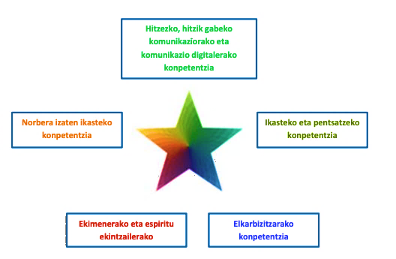
\includegraphics{zehar_konpe}
    \centering
    \par{Iturria: \citeauthor{ej2016curriculuma} (\citeyear{ej2016curriculuma})}
\end{center}

\ref{fig:zehar_konpe} irudian azaltzen den moduan, bost oinarrizko zehar konpetentzia daude dekretatuta. Zehar konpetentzia hauetatik, marko honetarako garrantzitsua dena hau da: hitzezko, hitzik gabeko komunikaziorako eta komunikazio digitalerako konpetentzia. Konpetentzia honen baitan biltzen diren helburuen artean, informazioaren eta komunikazioaren teknologiak modu sortzaile, kritiko, eraginkor eta seguruan erabiltzea dago bilduta, edo beste modu batera esanda, konpetentzia digitala (edo KD, laburtzeko) garatzea. Lan honen gai nagusia hau izanik, nahiz eta gaia ikuspuntu teknologiko batetik jorratu gaia, zeharkako konpetentzia bat izanik hezkuntza osoari eragiten dion zerbait dela ulertu behar da.

Bestalde, eta diziplina barneko konpetentzietan erreparatuz, teknologiarako konpetentzia da testu honekin jarraitzeko ulertu beharrezkoa. Esan den bezala, konpetentzia teknologikoa ingeniaritzan eta industrian erabiltzen diren prozesu eta metodologietan oinarritzen da, baina KDekin oso erlazionatua dagoen atal bat ere badauka konpetentzia honek: informazioaren eta komunikazioaren teknologiak (edo IKTak, laburtzeko). IKTak egungo gizarteko esparru orotan erabiltzen den teknologia da (\citeauthor{graells2000tic}, \citeyear{graells2000tic}). Teknologia hauek, sistema globalizatu batean aurkitzen direnez, multinazionalek garatzen dituzte, eta beraien etekina handitzeko daude garatuak.

Konpetentzia teknologikoa lantzerako orduan, hau da \citeauthor{ej2016curriculuma}k (\citeyear{ej2016curriculuma}) argitaratutako curriculum\footnote{}-ean azaltzen dena:

\begin{adjustwidth}{3em}{0pt}
“Produktu eta sistema teknologikoak zentzuz erabiltzea eta garatzea, jakintza teknikoak eta gainerako adarretako jakintzak era metodiko eta eraginkorrean aplikatuta, interesa duten egoerak ulertzeko eta konpontzeko edota produktu eta zerbitzu berriak eskaintzeko, eta lortutako emaitzen berri ematea, hobekuntza-prozesuekin eta erabakiak modu arduratsuan hartzeko prozesuekin jarraitzeko.”
\end{adjustwidth}

Honekin adierazi nahi dena da, hezkuntza teknologikoko prozesu eta jakintzak bigarren planora mugituz, jakintzaren erabilera kritikoan zentratzen dela konpetentzia garatzean landu nahi dena. Teknologiak gaur egungo gizartean duen pisuaz hitz egingo da, zergatia ulertzeko.

Kontzeptu honekin hasteko, ZTG mugimenduak lantzen dituen ideia nagusiak ulertzeak lagundu dezake. Mugimendu honek duen oinarria teknologiak gizartean duen eragina azpimarratzea da. Mundu globalizatu honetan, gizarteak teknologiarekiko duen dependentzia geroz eta handiagoa dela dirudi, \citeauthor{osorio2002educacion} (\citeyear{osorio2002educacion}) testuetan irakurri daitekeen bezala. Globaletik arlo lokalera itzuliz, dependentzia teknologiko hauen inguruko onurak eta kalteak bereizten jakitea garrantzitsua da, eta ikuspegi kritikoa landu behar da. XXI. mendeko euskal gizarte modernoak dituen erronken erroan aurki daiteke teknologia, zeharka baldin bada ere. Modu batera edo bestera, arlo teknologikoa inplikatuta dago erronka hauetan. Lehen hezkuntzatik datorren gazteak etorkizunean gizarteko erronketan inplikatuta egongo denez, ikuspuntu teknologikoa eta iritzi kritikoa garatzea beharrezkoa da.

Gazteek hezkuntza teknologikoa jasotzen hasi zirenetik, betidanik aipatu da teknologiaren ikaskuntza nola burutu behar den. Nahiz eta teknologia ikasgai bezala irakatsi, hastapenetatik argi izan den gauza da teknologia zeharka eragiten duen ikasgaia dela (\citeauthor{gilbert1995educacion}, \citeyear{gilbert1995educacion}). Azken finean, ezagutza zientifikoari oso lotuta dagoen gaia da, elkarbizitza ohikoa izanez, beraz garrantzitsua da ikasleengan lotura hauen ebidentzia adieraztea. Bestalde, aurrerapen teknologikoak hezkuntzan ere aplikatzen dira, eta aro digital berri baten aurrean aurkitzen da sistema. Eta hau, curriculumaren konpetentzia izaerarekin lotuz, islatuta geratzen da KDen garapenean zentratzen den atalean. Baina honekin jarraitzeko, beharrezkoa da XXI. mendeko euskal gizartearen erronkak ulertzea, eta nola islatzen den hau hezkuntza curriculumean.

Beraz, esparru bereko curriculumeko bi konpetentzia aztertu dira, eta konpetentzia hauetan iritzi kritikoa, neutraltasuna zein burujabetasuna aipatzen dira, baina edukiei begira horrelako lanketarik egiteko emaitzarik ez dagoela ikusten da. Hau honela izanda, bestelako markoetan aurkitu behar izaten da sakontzeko aukera. Jarraian aipatuko den hezitzaileen konpetentzia digitalerako Europar markoak\footnote{Ingelesez, \textit{European Framework for the Digital Competence of Educators}.} (edo DigCompEdu markoa) zerbait gehiago sakontzen du honen inguruan.

\section{Digitalizazioa}\label{sec:digitalizazioa}

Prozesu hau aurreko mendetik datorren joera bat da. Gizarteko alor guztietan aurki daitezke prozesu honen adierazleak, baina hasteko hezkuntzak jaso duen prozesua aztertuko da.

\subsection{DigCompEdu}\label{subsec:digcompedu}

Marko honek Europako hezitzaileen gaitasun digitala garatzeko esparru bat aurkezten du. Helburua, Estatu kideei laguntzea da beren herritarren gaitasun digitala sustatzeko eta hezkuntzaren berrikuntza bultzatzeko ahaleginetan. Markoak hezitzaileen gaitasun digitala sustatzeko, bai nazio, eskualde eta tokiko mailan egiten diren ahaleginak laguntzea du helburu, horretarako, erreferentzia-esparru komun bat eskainiz, hizkuntza eta logika partekatu batekin (\citeauthor{JRC107466}, \citeyear{JRC107466}).

Markoak Europar Batzordeko \textit{Joint Research Centre}-k (JRC) gauzatutako lanean du oinarria, hezkuntza, gazteria, kirol eta kultura Zuzendaritza Nagusiaren izenean.

DigCompEdu markoak Europako kide diren estatuetako kezkari erantzuten dio, hezitzaileen kezka propio bati, hain zuzen. Lanbide honen gaitasun digital multzo baten beharra argi manifestatzen da, teknologia digitalek duten ahalmena aprobetxatu ahal izateko. Honela, hezkuntzan hobekuntzak eta berrikuntzak gauzatuko dira.

DigCompEdu markoaren helburua da hezitzaileen gaitasun digitalerako dauden tresnei buruz hausnartzea eta hezkuntza-maila guztietako hezitzaileei beren gaitasun digital pedagogikoa ebaluatu eta garatzea ahalbidetzen dien eredu koherente batean sintetizatzea.

Hortaz, DigCompEdu-k ondorengo puntuetan azaltzen diren balore erantsiak eskaintzen ditu:

\begin{itemize}
    \item Maila guztietan hezkuntza-politikak bideratu ditzakeen oinarri sendo bat.
    \item Interesa ageri duten tokiko eragileei, beren beharrei egokituta dagoen tresna zehatz bat berehala garatzeko eredua, lan honetarako oinarri kontzeptual bat garatzeko beharrik gabe.
    \item Herrialdeen arteko praktika hoberenak trukatzen eta eztabaidatzen lagungarria izan daitekeen hizkera eta logika bateratu bat.
    \item Estatu kide, beste interes-talde eta beste edozein parte-hartzaileentzako erreferentzia-puntua, beren tresna eta esparruen osotasuna eta ikuspegia baliozkotzeko, bai oraingoak eta bai etorkizunekoak.
\end{itemize}

5.Irudian ikus daitekeen moduan, DigCompEdu markoak sei arlo ezberdin bereizten ditu, hezitzaileen gaitasun digitala nabarmentzen dituen hogeita bi konpetentziarekin osatuta.

\begin{center}
    \captionof{figure}{\textit{DigCompEdu arloak eta irismena}}
    \label{fig:digcompedu_arloak}
    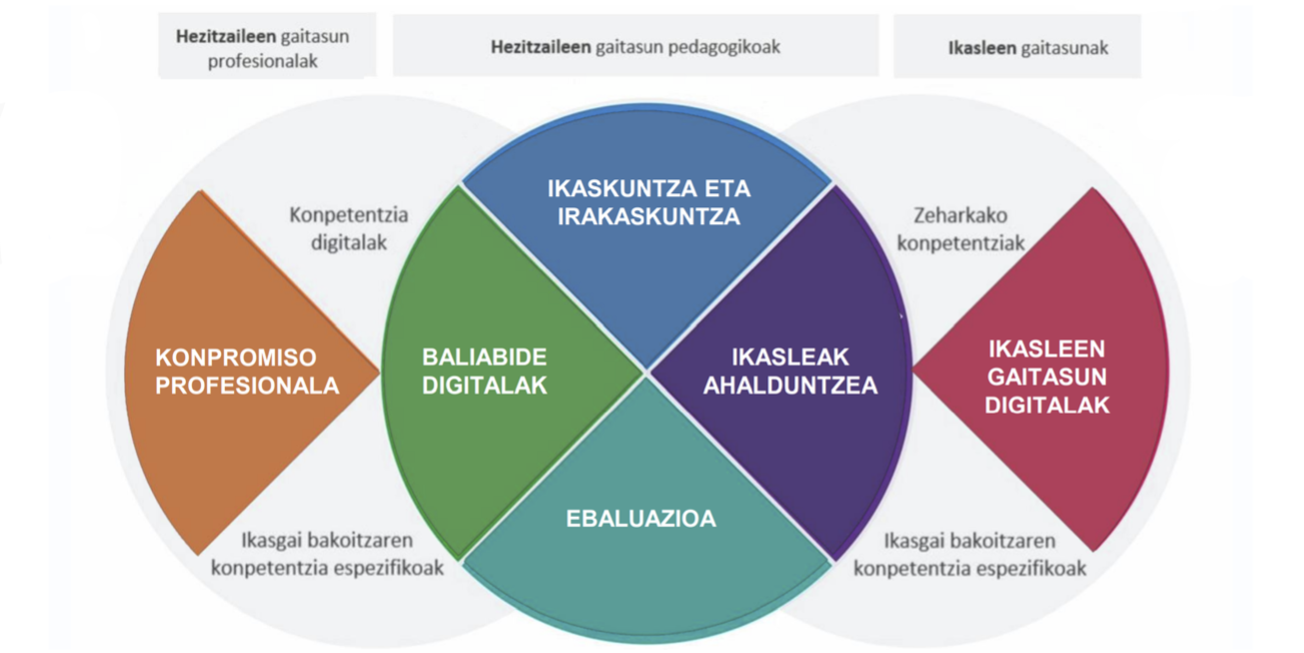
\includegraphics{digcompedu_arloak}
    \centering
    \par{Iturria: Sorkuntza propioa. Abiapuntua: \citeauthor{JRC107466} (\citeyear{JRC107466})}
\end{center}

\citeauthor{JRC107466}en \citeyear{JRC107466} testuan irakurri daitekeenez, irakasleek, gizarteko beste edozein pertsona bezala, gaitasun digitalak behar dituzte. Behar hau, gainera, garrantzitsuagoa da, ondorengo argumentuagatik:

\begin{adjustwidth}{3em}{0pt}
“Irakasleak eredu dira hurrengo belaunaldientzat. Hortaz, behar-beharrezkoa da gizarte digital batean aktiboki parte hartzeko herritar guztiek behar duten gaitasun digitala izatea irakasleek. Edonola ere, irakasleak ez dira ereduak soilik. Oroz gain, ikaskuntzaren gidari dira, edo, are sinplekiago, irakasle. Ikaskuntzan diharduten profesional gisa, ezinbestekoa da, bizitzarako eta lanerako beharrezkoak diren gaitasun digitalez gain, irakasleentzat espezifikoak diren gaitasun digitalak izatea, teknologia digitalak eraginkortasunez erabili ahal izateko irakasteko orduan. DigCompEdu esparruaren helburua irakasleentzat espezifikoak diren gaitasun digital horiek zehaztu eta deskribatzea da.”
\end{adjustwidth}

Beraz, hurrengo zerrendan bilduta daude marko honek biltzen dituen gaitasun digitalen zerrenda, 6 arlotan banatuta.

\begin{enumerate}
    \item arloa. Konpromiso profesionala: garapen profesionalerako, elkarlanean aritzeko eta komunikatzeko teknologia digitalak erabiltzea.
    \item arloa. Baliabide digitalak: eduki digitalak eskuratu, sortu eta partekatzea.
    \item arloa. Irakaskuntza eta ikaskuntza: irakaskuntzan eta ikaskuntzan teknologia digitalen erabileraren kudeaketa eta antolaketa.
    \item arloa. Ebaluazioa eta feedback-a: ebaluazioa hobetzeko teknologia eta estrategia digitalak erabiltzea.
    \item arloa. Ikasleak ahalduntzea: teknologia digitalen erabilera ikaslearen ikaskuntza propioaren baitan inklusioa, pertsonalizazioa eta konpromiso aktiboa areagotzeko.
    \item arloa. Ikaslearen gaitasun digitala sustatzea: ikaslearen prestakuntza, teknologia digitalak sormenez eta arduraz erabiltzeko, informatzeko, komunikatzeko, edukiak sortzeko, ongizaterako eta arazoen konponketarako.
\end{enumerate}

\citeauthor{JRC107466} (\citeyear{JRC107466}) argudioak erabiliz, 2. eta 5. arloetan banatzen da marko honen muina. Bi arloak elkarlanean irakasleen gaitasun digitalak aztertzen dituzte hezkuntza digital eraginkor, inklusibo eta berritzaileak sustatzeko. 1., 2. eta 3. arloek irakaskuntza prozesuko etapetan oinarritzen dira, eta teknologia digitalaren erabilera non eman daitekeen adierazi dezake. 5. arloa berriz, teknologiaren ikaslea erdigunean jartzeko ahalmena azpimarratzen du, eta marko honen zeharkako arlo gidatzailea dela esan daiteke.

DigCompEdu esparruak sei etapa deskribatzen ditu, irakasleek gaitasun digitalak garatu ahala igaro ohi dituztenak, irakasleei laguntzeko zer etapatan dauden identifikatzen eta zer pauso eman behar dituzten erabakitzen, beren gaitasuna hobetzeko.

\begin{itemize}
    \item Hasiberria (A1) eta Esploratzailea (A2): irakasleek informazio berria bereganatu eta oinarrizko jardunbide digitalak garatzen dituzte.
    \item Integratzailea (B1) eta Aditua (B2): irakasleek jardunbide digitalak aplikatu, zabaldu eta egituratzen dituzte.
    \item Liderra (C1) eta Aurrendaria (C2): irakasleek ezagutza partekatu, jardunbideak zalantzan jarri eta jardunbide berriak garatzen dituzte.
\end{itemize}

Posible da ekipo berean, profil edo maila desberdinetako irakasleak izatea eta bakoitzak bere paperean jardungo du. Adibidez, B1 mailako irakasle batek eduki digitalak bilatuko ditu eta talde berean, B2 mailako adituak, nolakotasuna adierazgarri moduan duena, integratzaileak aipatutako edukiak nola aplikatu adieraziko du. Talde berean, esploratzaile mailan dagoen irakasle bat balego, ikasle batek teknologia digitalak erabiltzeko orduan zein zailtasun izan ditzakeen identifikatuko du. Azkenik, talde horretan laugarren kidea C1 mailan badago, aurreko guztiari forma emango lioke, proiektua aurrera eramateko.

Hezkuntza zailak 5 erronka nagusi irudikatu ditu bere digitalizazio planean. Irakasleek zer motatako prestakuntza behar duten zehazteko, \citeauthor{larralde2021}-k (\citeyear{larralde2021}), galdetegi bat gauzatu zuen esparru publikoko irakasleekin. 3411 erantzunetatik, ondorengoak dira kezka gehien sortzen dituzten gaiak DigCompEduk bereizitako esparru bakoitzean.

Ia gehienek, prestakuntza etengabekoa behar duela izan adierazten dute. DigCompEdu markoaren baitan, atal bakoitzean emaitzarik adierazgarrienak adierazten dira. Adibidez, ikus-entzunezko baliabideak oso garrantzitsutzat jotzen dituzte irakasleak (DigCompEdu-ko 2. atala), metodologia aktiboen erabilera (DigCompEdu-ko 3. Atala) edota ebaluazio konpetentziala (DigCompEdu-ko 4. Atala). Aniztasuna eta diseinu unibertsala buruan duten beste kezka nagusietako bat da (DigCompEdu-ko 5. Atala) eta azkenik, ziber-bizikidetza, segurtasuna, eta teknologia digitalen erabilera osasuntsua (DigCompEdu-ko 6. Atala) (\citeauthor{larralde2021}, \citeyear{larralde2021}).

Beraz, hainbat aldiz aipatu den bezala, hezkuntzan digitalizazio prozesuaren agerpenak baliabide digitaletan dauka oinarria. Baliabide digital honek ulertzea beharrezkoa da hezkuntzan izan dezakeen eragina kritikotasunez aztertzeko.

\subsection{Baliabide digitalak}\label{subsec:baldig}

Baliabide digitalak irakasleen KDen parte bat dira, DigCompEdu markoan adierazita dagoen bezala. Hezkuntzan, irakasteko helburua duten tresna multzoari dagokionez, izendatze kontsentsu argirik ez da garatu, baina \citeauthor{pinto2012recursos}-ek (\citeyear{pinto2012recursos}) egindako definizioaz baliatuz, material digital oro, hezitzeko helburuarekin erabiltzen dena, baliabide digitala da.

Definizio honetaz baliatuz, multzo honetan zerrendatu ditzakegu heziketa prozesurako erabilgarriak diren dokumentu, multimedia artxibo, software zein web orrialde oro. Baina multzo honen barruan, sailkapen kriterio asko erabili daitezke. Dokumentu honetan erabiliko dena hurrengoa da: baliabide libreak eta baliabide pribatiboak.

\subsubsection{Software librea}\label{subsubsec:softwarelibre}

Baliabide libre eta pribatiboen arteko bereizketa egiterako orduan, \citeauthor{stallman2002}-ek (\citeyear{stallman2002}) sortutako manifestura jo behar da. Softwarean oinarritzen den mugimendu honek argi uzten du zer den librea eta zer ez. Software librea banatzeko (erabilera komertziala eginez ala ez), aztertzeko eta eraldatzeko askatasun osoa duen software oro da. Software askea, komunitate batek garatutako softwarea izan ohi da, etekinak lortzeko asmorik gabe: egoa gizentzea da helburu bakarra. Software pribatiboak berriz, lizentziapeko babesa izaten du. Lizentzia eskuratzean (ordainpekoa izanez gehienetan) softwarearen erabilera egiteko eskubidea eskuratzen da, baina ez da aztertu, eraldatu eta banatzeko eskubiderik bermatzen. 

\subsubsection{Lizentziak}\label{subsubsec:lizentzia}

Lizentziak, aurreko paragrafotik eratorri daitekeen definizioan oinarrituta, baliabide digital bat erabili edo banatzeko baimena da. \citeauthor{labrador2012}-en (\citeyear{labrador2012}) hitzetan, lizentzia irekiak edo itxiak izan daitezke, eta bakoitzaren barruan sailkapen sakonago bat dago, baina dokumentu hau ulertzeko libreen artean bi mota ikusiko dira.

Lizentzia libreen barruan, alde batetik, lizentzia guztiz libreak edo Creative Commons oinarripean banatzen diren lizentziak ditugu, era askean erabili eta banatu daitezken baliabideak izanez (nahiz eta baldintza batzuk izan). Bestalde, baliabide semi-librea daude, eta hau, nahiz eta asmo komertzialetarako izan, doan eta libre banatzen da. Honekin lotuta, azken urteetan baina, termino berri bat hasi da agertzen industrian: hezkuntzarako lizentziak. Softwarea erabiltzeko lizentzia mota honen berezitasuna, lizentzia komertzialekin alderatuta, ikasle zein irakasleentzat doakoa dela da. Lizentziatutako tresna hezitzeko erabiltzen bada doako da eta inolako eragozpenik gabeko erabilera egin ahal izango da, beti ere etekin ekonomikorik ez bada lortzen lizentzia honetatik eratorritako produktuekin Baina enpresa handien interesa ez da kapitala metatzen jarraitzea baino besterik (\citeauthor{marx1867}, \citeyear{marx1867}). Beraz, enpresa batek zerbait doan ematean, interes bat izango du. Kasu honetan, eta \citeauthor{brouilette2002}-ek (\citeyear{brouilette2002}) adierazten duten moduan, ikasleak ekosistema bateko softwarea erabiltzera bultzatzean, lan mundura integratzean software hau erabiltzen jarraitzeko joera izango dute. 


\subsubsection{Baliabide libreak}\label{subsubsec:baliabidelibre}

Hau baliabide digitaletara estrapolatuz, baliabide digital bat librea izango da edonork erabili ahal badu, nahi den moduan interpretatu eta banatzeko (\citeauthor{butcher2011basic}, \citeyear{butcher2011basic}). Baina baliabide digitalen eremuan, adierazle berri bat sartzen da askatasun hau ebaluatzeko unean. Jakina da GAFAMek esku hartze handia dutela hezkuntzan, ikustekoa da \citeauthor{joseph2019toward}-ek (\citeyear{joseph2019toward}) egindako kasu ikerketa, non proiektu batetik bost enpresa hauek ateratzen saiatu ziren, arrakastarik gabe. Landutako eztabaidan, enpresa hauen zilegitasuna jartzen da zalantzan, hauek tresna digital ugari eskaintzen dituzte baliabide digitalak sortu eta partekatzeko. Baina enpresa hauen negozio modeloa ez da hain argi geratzen praktika hauetan, eta horregatik sortzen dira zalantzak “baliabide digital libreak” deitura eskuratzeko orduan. Jarraian enpresa hauek sortzen dituzten datuak aztertuko dira, hezkuntzarengan izan dezakeen eragina ikusteko.

\subsection{Aztarna eta profil digitala}\label{subsec:aztarna}

KDen garapenaren garrantzia argi geratu da, gaur egungo bizitzaren pertzentil handi bat mundu digitalean gertatzen da eta. Gizarte garaikidean, egunero mugikorrerako aplikazio (\textit{app} bezala ezagutuak) berriak sortzen dira, orain dela asko irudika-ezinak ziren esparruetan teknologia digitala integratuz (\citeauthor{vervier2017perceptions}, \citeyear{vervier2017perceptions}). Finantzak, osasuna, kirola… hainbat dira eredu modura erabili daitezkeen esparruak, eta hezkuntza ere hauekin batera sartu daiteke, multzo berdinean.

Digitalizazioak hezkuntzan dituen abantailen zerrenda amaiezina da, baina \citeauthor{cobos2009}-ek (\citeyear{cobos2009}) zerrendatu zuten moduan, motibazioa, interesaren sustaketa eta bestelako onurak distrazio, partzialitate falta eta isolaketa moduko kontrako argudioekin egiten dute topo. Aurkako argudioen artean baina, bada bat gizarteko eremu guztietara aplikatu daitekeena. \citeauthor{vervier2017perceptions}-en (\citeyear{vervier2017perceptions}) hitzetan, gaur egungo bizitza mundu digital batera konektatua bizitzeak aztarna digitalak sortzen ditu. Aztarna digitala mundu digitalean nabigatze hutsagatik sortzen diren datuak dira, eta multinazional handiek, aurrez aipatu den bezala, publizitatea egiteko erabiltzen dute, etekin handiak lortuz. Hau gizartearen kezka handi bat dela diote (Bansal et al., 2010; Rainie et al., 2013; Data Protection Eurobarometer, 2015; TRUSTe, 2014, aipud \citeauthor{vervier2017perceptions}, \citeyear{vervier2017perceptions}), eta kontzientzia maila altu bat garatzea da espero den joera. Baina \citeauthor{norberg2007privacy}-ek (\citeyear{norberg2007privacy}) aipatutako paradoxan, hau ez da horrela islatzen. Gizarteak geroz eta datu gehiago sortzen ditu multinazionalen mesedetan.

Hau dela eta, profil digitalak sortzea da multinazional hauen joera. \citeauthor{azucar2018predicting}-ek (\citeyear{azucar2018predicting}) burututako profil digitalak multzokatzeko sistema batean aipatzen duten bezala, profil digital bat pertsonalitate desberdinak multzokatzen dituen datu multzoak dira. Profil digital desberdinak mundu digitalaren erabilera pertsonalizatu ahal izateko da, eta printzipioz onuragarria izan daitekeen arren, erabilera nagusia publizitate kanpaina zehatzak egiteko da.

Atalaren hasieran aipatu den moduan, KDaren garapena garrantzitsua da. Baina garrantzitsua da ere kontzientzia hau garatzen joatea konpetentzia garatuz doan heinean. Aztarna digitala mundu digitala erabiltzen hasten den unetik sortuz doa, eta konpetentzia honen barnean bilduta egon beharko da kontzientzia kritikoaren garapen hau. Gaur egungo gazte bat, IKTak erabiltzen hasten den unetik, aztarna digital bat sortzen hasiko da, profil digital baten barruan kokatzen joango dena. Jakin gabe, eta gutxinaka gutxinaka, bere etorkizuna mugatuz joango den datu kopuru handi bat joango da sortzen, honetaz kontzientzia izan gabe (\citeauthor{wook2019awareness}, \citeyear{wook2019awareness}).

\subsection{Baliabide libreen antolaketa}\label{subsec:baliabide_antolakuntza}
Baliabide digitalekin amaitzeko, hauek jarraitzen duten antolaketa ulertu behar da, hau baita baliabide libreen desabantaila nagusia. GAFAM enpresen baliabidea, enpresa beraren zerbitzarietan egoten dira instalatuta, eta erabiltzaileak modu erosoan erabili ditzake inongo instalaziorik egin gabe (\citeauthor{burger2019distributed}, \citeyear{burger2019distributed}). Baliabide libre baten kasua desberdina da. Diru sarrerarik ez duten erakundeak izanda, ezinezkoa da zerbitzua eskaintzeko beharrezkoak diren zerbitzariak ordaintzea (plan \textit{premium} bat eskaintzeke), eta erabiltzaile bakoitzak bere instalazioa burutu behar du erabili baino lehen. Nahiz eta ikastetxeetako infraestrukturan zerbitzariak badauden, zerbitzu hauek kudeatu eta mantentzea ez da erraza izaten, beraz aurkako argudio moduan erabili daiteke.

\section{Irakasleen formakuntza}\label{sec:formakuntza}

Etengabeko transformazioan dagoen gizartean eta eraldaketa geroz eta abiadura azkarrago batean gertatzen den honetan, hezkuntza sisteman aldaketak gutxi dira eta oso motel doaz. Ikasleak hezkuntzaren protagonista eta oinarria badira ere, askotan hauen egitekoaren aldaketa etengabean jartzen da arreta. Fokua ikaslearengan jarri beharrean, askotan balore, ezagutza eta konpetentziak garatzen laguntzen dizkien irakasleengan jartzen bada eta aurretik aipatutako puntua kontuan hartuta, hauen prestakuntza eta formakuntzarako behar etengabea azaltzen da. \citeauthor{bosch2018konpetentzia}-ek (\citeyear{bosch2018konpetentzia}) ondorioztatu zuen, gizakion heziketa ez da sekula amaitzen eta, irakasleen kasuan, etengabeko prestakuntzan dihardute.

Berrikuntza batek aldaketak eskatzen dizkio eskolari, bai baliabide, material, eta formakuntzan. Baina hezitzaileak ez formatzeko arrazoiak ere beste hainbeste izan daiteke. \citeauthor{perrenoud2001formacion}-ek (\citeyear{perrenoud2001formacion}) dioen moduan, eskolaren kontzepzioa eta irakaslearen papera honetan ez doaz bat askotan. Aurrekoaren ondorioz, irakasleen prestakuntzaren inguruko konfrontazioek askoz oinarrizkoagoak diren dibergentziak ezkuta ditzake. Zoritxarrez, ezin da defendatu Estatu guztiek irakasle, intelektual, profesional eta humanistak, gogoetatsu eta kritikoak prestatu nahi dituzten hipotesia.

Hau horrela, berrikuntzarako eta eraldaketarako beharra irakaslearen nahi eta gogoeta propiotik ateratzen den ekintza da. Baina adibidez, \citeauthor{perez2014irakasleen}-k (\citeyear{perez2014irakasleen}) dio, hezkuntzako eragile garrantzitsuenetako bat irakaslea izanik, pentsaezina litzatekeela eskolan berrikuntza bat egitea beraiek kontuan izan gabe, beraiek baitira aldaketa horren eragile nagusiak: aldaketa horren aurrean eragile horien jarrera ezkorra edo desegokia izatea arazo handi bat izango litzateke konpetentzia digitalaren garapena sustatzeko. \citeauthor{arroyo2017competencias}-k (\citeyear{arroyo2017competencias}) dioen bezala, irakasleak argi izan behar du edukietan oinarritutako irakaskuntzari buelta bat emateko, bera dela irakaskuntza-metodo berrira egokitzeko konpetentzia berriak landu behar dituen lehenengo pertsona.

\citeauthor{bosch2018konpetentzia}en (\citeyear{bosch2018konpetentzia}) ondorioarekin bat eginez, irakasleen laneko atal handi bat da norberarena ez den beste arloekiko interesa piztea, eta berrikuntzei ateak irekitzeko jarrera sustatzea. Hezkuntzan aldaketak uneoro gertatzen dira, eta, hau ez bada onartzen, ikasleei datozen gauza berri horiek ezagutzeko aukera ukatzen da.

\subsection{Praktika komunitate profesionalak}\label{subsec:pkp}

Irakasle lanbidea lan kolektibo bezala ulertzen bada, indibidualismotik komunitaterako saltoa ematea beharrezkoa da. Espezialitateko irakasle izatetik haratago, tutore izateak duen pisua eta bizi garen gizartean bertako eta bartakoentzako irakaskuntza garatzeko. Horregatik, PKP markoak batzen dituen gakoak, ikastetxe komunitaterako ezinbestekoak dira.

\citeauthor{dufour1998professional}-en (\citeyear{dufour1998professional}) arabera, eskolaren hobekuntza iraunkor eta nabarmenerako estrategiarik itxaropentsuena, ikastetxeko langileak ikaskuntza-komunitate profesional gisa funtzionatzeko gaitasuna garatzea da. Hori dela eta, PKP ereduak, profesionalei praktika berriak ikasteko eta ezagutza berriak sortzeko aukera ematen du, ikasleen ikaskuntza hobetzeko helburuarekin.

PKPak, berrikuntza iniziatiba hutsa izatetik, eskoletako egitura euskarri izatera bihurtzen dira, hauen etengabeko transformazio eta eraldaketa propioa bultzatuz. (\citeauthor{morrissey2000professional}, \citeyear{morrissey2000professional}). Honek eragin zuzena izango du prozesu honetan protagonista diren ikasleen hezkuntza eta ikaskuntzan, baina aldaketa honen eragile diren irakasleetan baita.

Ikasleak ardatz hartuta, PKP baten helburu nagusia \citeauthor{dufour2004whatever}-en (\citeyear{dufour2004whatever}) arabera, ikasle guztiak ikasten dutela ziurtatzea da, elkarrekintza kultural eta emaitzetan fokua jarriz. Horregatik, irakaslearen konpromisoa, ikasle guztien “hezkuntza arrakasta” lortzea da, hau da, ikasten ari direla ziurtatzea.

Ezin daiteke ulertu ikaslearen ikaskuntza era eraginkor batean emateko baliabideak sortzea eta mantentzea, irakaslearen garapenerako baldintzak ematen ez badira. \citeauthor{bolivar2012melhorar}-ek (\citeyear{bolivar2012melhorar}) dioenaren arabera, askotan ikasleentzako ikaskuntza-kultura berri bat sortzea proposatzen bada, kontuan izan behar da hori ez dela guztiz gertatuko irakasleentzat ikaskuntza kultura propio bat sortzen ez bada. Horregatik, eskola “birkulturatzeaz” geroz eta gehiago hitz egiten da, ikas-komunitate profesional gisa moldatzeko. Honek, irakaslearen formakuntza jarraia behar duela adierazten du.

\subsubsection{Praktika Komunitate Profesional eraginkorrak}\label{subsubsec:pkpe}

Praktika komunitatea, gai batekiko kezka, problematika multzo edota gai zehatz batzuekiko grina partekatu eta etengabeko interakzioen bitartez, beren ezagutzak eta esperientziak sakontzen dituzten pertsona taldea da (\citeauthor{wenger2002cultivating}, \citeyear{wenger2002cultivating}). Irakasle eta ikasleen praktikan eta hauen berrikuspenean foku berezia jartzen da eta eskolak ulertzeko eran bereziko aldaketa nabarmentzen da. 

PKP baten elkarrekin lan egiten duten giza talde bat eraldatzen duten ezaugarriak zehazten dira, eta puntu hauetan daude definituak (\citeauthor{louis1995professionalism}, \citeyear{louis1995professionalism}; \citeauthor{stoll2007professional}, \citeyear{stoll2007professional}):

\begin{itemize}
    \item Balore eta ikuspegi partekatuak: ikastetxearen helburuen baitan eraikitako eta partekatutako balore eta ikuspegien multzoa. Ikaslearen ikaskuntzan konprometitua eta bideratua, non espektatiba altuak nagusi diren eta hobekuntzarako ohitura bat ematen den.
    \item Eskaintzen den hezkuntza hobetzeko ardura kolektiboa: langileak ikasle guztien ikaskuntzarekin konprometituta daude eta hauen arten presio txiki bat ematen da irakasleak guztiak norabide berean joka dezaten.
    \item Ikasleen ikaskuntzara eta irakasleen egiteko onenera bideratuta,: ikasleen ikasteko aukerak areagotzeko eginkizunean oinarrituta; horrek irakasleak, plangintza, lan eta ekipoko ikaskuntzaren bitartez, etengabeko ikaskuntzarekin kezkatuta daudela adierazten du.
    \item Lankidetza eta praktikaren despribatizazioa: elkarrekiko laguntza eta antolakuntzaren ikaskuntza ahalbidetzen duen lankidetza-harremanak. Bakoitzak egiten dakiena partekatzeko, besteei laguntza eskatzeko eta emateko borondatea ematen da harreman profesionalen baitan, non lankideak ezagutza eta feedback iturri kritiko bihurtzen diren.
    \item Banakako eta taldekako ikaskuntza profesionala: langile guztiak, aholkulariak barne, ikaskuntza profesionalaren hobekuntzan inplikatuta daude eta hau baloratzen dute, helburu horretara bideratutako jarduerak aurrera eramanez. Praktikaren hausnarketa garatzen da, ikaskuntza eta irakaskuntzari buruzko ikerketa bidez (adibidez, elkarren arteko behaketa, autoebaluazioa, ikerketa ekintza), datuak aztertu eta hauek erabiltzen dira hobekuntzarako.
    \item Zabalkuntza, sareak eta aliantzak: kanpoko ekimenak, barnean gertatzen dena aztertzeko erabiltzen dira. Langileak aldaketarako eta beste ikastetxe edo erakunde batzuekin sareak edo aliantzak ezartzeko irekita daude, ikaskuntzan elkarri laguntzeko.
    \item Komunitate inklusiboa, elkarrekiko konfiantza, errespetua eta laguntza: lan harremanak elkarrekiko konfiantzan, errespetuan eta laguntasunean oinarritzen dira. Kide guztiak partehartzaile aktibo sentitu daitezen berebiziko arreta jartzen da. Desberdintasun indibidualak eta desadostasunak taldearen garapena ahalbidetzen duten hausnarketa kritiko baten barruan onartzen dira, norbanakoaren eta komunitatearen arteko dikotomiarik existitzen ez delarik.
\end{itemize}

\subsubsection{Oinarriak}\label{subsubsec:pkp_oinarri}
PKPak definitzeko \citeauthor{dufour2004whatever}-ek (\citeyear{dufour2004whatever}) ikaslearen jardueran oinarritzen diren ondorengo hiru ideiak definitzen ditu:

\begin{itemize}
    \item Ikasle guztiek ikasten duten ziurtatzea: ikasle batek zailtasunak dituen momentuan, zeregin horri erantzuteko komunitate zentzua aktibatzen da.
    \item Kolaborazio kultura: kolaborazioa, prozesu sistematiko bat da, irakasleek taldean lan egiten dute haien praktika aztertu eta hobetzeko bidean.
    \item Emaitzetan fokua: PKPak errutinako lanaren parte dira, eta ikasleen errendimendua hobetzeko ahalegin bateratuan lan egiten dute. Irakasle talde bakoitzak, ikasleen uneko lorpen-maila identifikatzeko etengabeko prozesu batean parte hartzen du, egungo edo uneko egoera hobetzeko helburuak ezarriz eta aurrerapenaren datu eta proba periodikoak emanez.
\end{itemize}

Harreman kooperatiboko testuinguruak garatzean oinarritzen da, non hezkuntza eragile ezberdinek (barnekoak zein kanpokoak), beren garapen profesionalerako, profesional konprometituen komunitatearen baitan, eskola esparruaren berreraikuntza sozial eta kulturalean lagun dezaten (\citeauthor{bolivar2012melhorar}, \citeyear{bolivar2012melhorar}). 

Helburua beraz, ikastetxearen komunitate sentimendua sustatzeko, irakasleen eginkizunak eta lana birdiseinatzea da. Kolaborazio eta elkargoko harremanen bitartez, irakasleak erakundearen garapenean inplikatuz, ikastetxean adostutako eginkizunekin zentroko pertsonala konpromiso batera bultzatuz. Proiektu bateratuetan lan egitea, indibidualismotik komunitate profesionalaren trantsizioa egiteko baliabide aproposa izan daiteke.
\chapter{Formakuntza saioa}\label{cha:formakuntza}

Behin formakuntza saioa oinarritzen den marko teorikoa osatuta, ondorengo atalean, honen diseinua gauzatzen da. 

\section{Formakuntzaren aurkezpena}\label{hemendik aurrera ez dao labek gehixau, pereza maxima}

Praktika Komunitate Profesionalen markoan oinarritutako formakuntza saio hau, esparru publikoko, DBH eta Batxilergoko irakasleei zuzendua dago, Informazio eta Komunikazio Teknologien (IKT) irakaskuntza modu zuzen batean etapa horietan lantzen delako gehienbat. Formakuntza honekin lortu nahi dena, ikastetxeetan erabiltzen diren baliabide digitalen irakurketa kritiko bat egitea da, inguratzen dituzten elementuen ondorioen jakitun izateko. Baita ere, burujabetza digitalaren filosofia ezagutaraztea eta horretan lanean dauden eragile/elkarteak aditzera ematea eta hauek proposatzen dituzten erabilera libreko softwareetan irakasleak trebatzea, ondoren jakintza eta lan egiteko modu hauek ikasgeletan transmititzeko. 

Formakuntza hau 5 saio nagusitan antolatua dago, bakoitza 2-3 orduko iraupena dutenak. Saioak hilabeteko lehen astelehenetan izango dira. Modu honetara, saio bakoitzetik bestera hilabeteko tartea egongo da ikasitako edukiak ikastetxean aplikatzen hasteko eta aldi berean denbora tarte horretan emandako bilakaeraren balorazio bat egiteko. Bertan, metodologia aktiboak erabiliz talde eta banakako lanketa, hausnarketa eta dinamikak eramango dira aurrera.

Edukien aipamen bat egitearren, lehen saioan GAFAM enpresek hezkuntzan aurrera eramaten duten eskuhartzea landuko da. Bigarrenean, burujabetza digitalaren kontzeptuan sakonduko da, horretan lanean dauden elkarteak ezagutaraziz eta hainbat adibide konkretu ikusiz. Hirugarren formakuntzan, software libreen gaian sakonduko da, zer diren, zertan oinarritzen diren eta non aurki daitezkeen azalduz eta laugarren saioan, hauetan trebatzea izango da asmoa. Azkeneko saioan, hausnarketa eta ebaluaziorako tartea irekiko da.

\section{Helburuak}

Formakuntzaren helburu nagusia, gaur egun ikastetxeetan ematen den digitalizazio prozesuaren bilakaeraren aurrean irakasleak hausnarketa kritikora bultzatzea. Digitalizazio prozesu honen norantza ikusita, burujabetza digitalerako bidean urratsak emateko asmoz, baliabide digital libreetan trebatuko dira saio hauetan zehar.

Helburu nagusia betetzeko bidean, hainbat helburu espezifiko definitu dira, formakuntzan zehar landuko diren edukiekin lotura zuzena dutenak:
\begin{itemize}
    \item Hezkuntza mundura hurbildu eta geratzeko etorri diren GAFAM enpresa multinazionalen ekosistema digitalak ikastetxeetan txertatzeko asmoak ezagutzea eta EAEko hezkuntza sistemaren eta gure ikasleen eskubideak urratzeak duen eraginaz ohartu eta hausnartzea.
    \item Egungo hezkuntza sisteman GAFAM enpresen esku hartzeari aurre eginez eta burujabetza digitalera bidean alternatibak planteatuz lan egiten duten eragile eta proiektuak ezagutarazi eta hauek aurkezten dituzten proposamenen inguruan hausnartu.
    \item Gaitasun eta trebeziak lortzetik haratago, irakaslea teknologia digitaletan ahalduntzea. Horretarako, hezkuntzan erabiltzen diren baliabide digitalak zerrendatzea eta hauetan enpresen eskuhartzea identifikatzea. Baliabide alternatibo libreak aurkitzea eta aurkitzen jakitea (burujabetza garatzea). Alternatiba nagusien erabileran trebatzea.
    \item Saioen artean definitutako helburuetan fokua jarriz, irakasle mintegiko kideen artean jakintzak partekatzea, komunitate profesional bat eratzen joanez eta aldi berean, emandako aurrera pausuen gaineko balorazioak eginez.
    \item Hezkuntza curriculumean bildutako KDen harira, garatutako kontzientzia hau ikasleen formakuntzan islatzea, baliabide digitalak erabiltzerakoan, hausnarketa hauetara itzuliz.
\end{itemize}

Helburu hauek lortzeko, formakuntza saioan landuko diren edukiak finkatuko dira jarraian. Eduki hauek formakuntza saioaren hiru ardatzetara orientatuta joango dira.

\newpage
\section{Edukiak}

Formakuntza saio honetan, 3 ardatz bereizi daitezke. Alde batetik, hezkuntza munduan esku hartzen duten enpresa pribatuen ezaugarritzea egingo da. Ondoren, enpresa hauen eskuhartzea murrizteko dauden joerak ezagutuko dira. Azkenik, joera horiek oinarritzen diren tresna libreetan trebezia garatuko da.

\begin{enumerate}
    \item Hezkuntza sisteman esku hartzen duten enpresen ezaugarritzea.
    \begin{enumerate}
        \item GAFAM enpresak ezagutu.
        \item GAFAM enpresen eskuhartzea eta bilakaera hezkuntzan.
        \item Multinazional hauen azaleko zein ezkutuko helburuak ezagutu, hezkuntza sistemari dagokionez.
        \item EAEko hezkuntza sistemako panoramaren diagnosia GAFAM enpresekiko
        \item Ikastetxeetara hurbilpena eta ikaslean fokua jarriz egungo egoeraren hausnarketa kritikoa garatu.
\end{enumerate}
    \item Hezkuntzako eredu digitalari aurre egiten dioten planteamenduen ezaugarritzea eta hauen jarduna EAEn.
    \begin{enumerate}
        \item Burujabetza digitalaren ideia ezaugarritu.
        \item Mugimendu horretan lanean dauden elkarte eta eragileak ezagutu eta hauen bilakaera aztertu (bertakoak eta atzerrikoak).
        \item EAEn aurretik eramandako proiektu/lan/aurrera-pausuak arakatu.
        \item Ikastetxeko azpiegitura digitalaren diagnosia definitu burujabetza mailarekiko.
\end{enumerate}
    \item Hezkuntzaren arlo digitalaren pribatizaziorako joeraren aurkako tresna eta baliabideak eskuratu.
    \begin{enumerate}
        \item Baliabide digitalen jatorria aztertzen jakin, erabiltzen diren baliabideak identifikatu.
        \item Alternatiba libreak ezagutu eta erabiltzeko joera bultzatu.
        \item Tresna pribatiboak erabiltzeko unean, izaera kritikoa landu.
        \item Software libretik datorren ideologia transmititu.
        \item Tresna erabilgarrietan trebatu, aldaketara pausua ematera bultzatu. 
        \item Irakaskuntza komunitatean tresna hauek zabaldu.
\end{enumerate}
\end{enumerate}


\section{Metodologia}

Hilabeteko tartea egongo denez saioen artean, garrantzitsua da jarraikortasuna bermatzea. Honetarako, aplikatuko den zentrotik arduradunak izendatuko dira, eta formazio guztira etorri beharko dira. Gogorarazi behar da formakuntza honen helburuetako bat PKPa eratzea dela, beraz arduradun hauek egunerokotasunean beste irakasleak komunitatean integratzeko betebehar batzuk izango dituzte. Hau ahalbidetzeko, irakaslegoaren \%40a bertaratzea espero da (20 irakaslerentzako prestatua dago formakuntza saioa), eta gutxienez departamentu bakoitzeko pertsona bat izatea lagungarria izan daiteke.

Lehenengo saio eta bigarren saioaren amaieran behaketa taulak sortuko dira, ikastetxearen diagnosia egiteko. Behaketa taula hauek saio bakoitzeko teoriarekin beteko dira, eta ikastetxearekiko izaera kritikoa izango dute. Hurrengo hilabeteko saioaren hasieran, behaketa taula aztertu eta ondorioak aterako dira, eta saio bakoitza ondorio hauetatik hasita birbideratuko da.

Hirugarren saioaren amaieran, ikastetxean egin daitezkeen aldaketa batzuk proposatuko dira. Ez du zertan errealista izan behar, laugarren saioan hausnartu eta epe luzerako plangintza bat finkatzeko balio izango du eta. Epe luzerako plangintzaren muina ikastetxe librezalearen kultura sortzea izango da.

Honetaz gain, DigCompEdu markoan oinarrituta, irakasleen hasierako konpetentzia digitalak neurtuko dira. Horretarako, eskaintzen den formularioa beteko da eta baliagarria izango da formazioan zehar maila altuena duten irakasleak IKTko arduradun bezala izendatuak izateko. Prozesu honetan zehar sortu daitezkeen zalantzak arduradun hauei komunikatuko zaizkie, eta hauek izango dira laguntzaile lana egingo dutenak (jakitun batekin kontaktuan jarriz edo beraien kabuz informazioa bilatuz).

Taldekatzerako orduan, pertsonen digitalizazio maila kontutan izango da. Aberasgarriagoa izan daiteke maila desberdinetako irakasleak elkarlanean aritzea, baina taldean DigCompEdu markoan “lider” rola duten irakasleak izateak gauzak erraztu ditzake. Hau dela eta, talde orokorraz gain, lau pertsonako “talde txikiak” sortuko dira, dinamiketan zehar erabiliko direnak.

\section{Denboralizazioa}

Irakasleei bideratutako formakuntza saio hau denboran zehar \ref{tab:plangintza} taulan ikusten den moduan antolatu da. 5 atal nagusiz osatua dago, eta atal bakoitza hilabeteko lehen astelehenetan burutuko da, honako gai desberdinak landuz. Irailetik aurrera hasiko da, ikasturtean zehar duen eraginaren gogoeta bultzatu nahi da eta.

\begin{center}
    \captionof{table}{\textit{Formakuntza saioaren plangintza}}
    \label{tab:plangintza}
    \begin{tabular}{|p{4,75cm}|p{9cm}|}
        \hline
        \rowcolor[HTML]{D9D9D9} 
        \textbf{DENBORALIZAZIOA} & \textbf{GAITEGIA}
        \\ \hline
        IRAILA → 1.saioa & GAFAM enpresen esku-hartzea hezkuntzan
        \\ \hline
        URRIA → 2. saioa & Burujabetza digitala, bide horretan lan egiten duten elkarteak eta hauen   proiektuak.
        \\ \hline
        AZAROA → 3. saioa & Tresna digital alternatiboak aurkitzen trebatu
        \\ \hline
        ABENDUA → 4. saioa & Baliabide digital libreetan trebatu
        \\ \hline
        URTARRILA → 5. saioa & Autoebaluazioa eta formakuntzaren ebaluazioa
        \\ \hline
    \end{tabular}
\end{center}

Saio bakoitzak 2-3 ordu bitarteko iraupena izango du eta saio bakoitzetik bestera hilabete bateko tartea egongo da. Formakuntza antolatzeko modu honen arrazoi nagusia saio bakoitzean eskuratutako ezagutzak ondoren ikastetxean lurreratzeko denbora edukitzea da, hau da, beste irakasleei ezagutza hauek transmititzea eta arlo honen progresurako bide orri bat diseinatzea beharrezko eztabaidak emanez. Gainera, lehen eta bigarren formakuntzetan behaketa taula ezberdinak prestatuko dituzte ondorengo hilabetean ikastetxeko egoera aztertzeko. Beraz, horretarako ere denbora behar da.

Horrez gain, behaketa taulako edukiak eta bertatik ateratako ondorioak mahaigaineratu eta horien inguruan hausnartzeko tarteak irekiko dira, taula osatu eta hurrengo formakuntza saioan partekatu eta talde gogoetak egin ahal izateko. Azken finean formakuntza saio guztiek elkarren artean lotura dute eta taula horietako edukia ezinbestekoa da ondorengo saioetarako oinarri moduan.

Jarraian, \ref{tab:denboralizazioa}. taulan, saio bakoitzaren denboralizazioa aurkitu daiteke. Saio bakoitzak hainbat fase izango ditu, helburu desberdinekin. Fase bakoitzak, aldi berean, dinamika ugari izango ditu.

\newpage
\begin{center}
    \captionof{table}{\textit{Formakuntza saioaren denboralizazioa}}
    \label{tab:denboralizazioa}
    \begin{tabular}{|p{3cm}|p{3cm}|p{3cm}|p{3cm}|p{3cm}|}
        \hline
        \rowcolor[HTML]{D9D9D9} 
        \textbf{1. SAIOA} & \textbf{2. SAIOA} & \textbf{3. SAIOA} & \textbf{4. SAIOA} & \textbf{5. SAIOA}
        \\ \hline
        \makecell{\textbf{0. Fasea:}\\
        Dinamika I:\\(15 min.)\\
        Dinamika II:\\(5 min.)} & 
        \makecell{\textbf{4. Fasea:}\\
        Dinamika IX:\\(10 min.)\\
        Dinamika X:\\(30 min.)} & 
        \makecell{\textbf{7. Fasea:}\\
        Dinamika XV:\\(10 min)\\
        Dinamika XVI:\\(20 min.)} &
        \makecell{\textbf{10. Fasea:}\\
        Dinamika XXI:\\(10 min)\\
        Dinamika XXII:\\(20 min.)} & 
        \makecell{\textbf{12. Fasea:}\\
        Dinamika XXV:\\(10 min)\\
        Dinamika XXVI:\\(30 min.)\\
        Dinamika XXVII\\(30 min.)}
        \\ \hline
        \makecell{\textbf{1.Fasea:}\\
        Dinamika III:\\(10 min.)\\
        Dinamika IV:\\(25 min)} &
        \makecell{\textbf{5. Fasea:}\\
        Dinamika XI:\\(30 min.)\\
        Dinamika XII:\\(25 min.)} &
        \makecell{\textbf{8. Fasea:}\\
        Dinamika XVII:\\(20 min.)\\
        Dinamika XVIII:\\(30 min)\\
        Dinamika XIX:\\(60 min.)} &
        \makecell{\textbf{11. Fasea:}\\
        Dinamika XXIII:\\(60 min.)\\
        Dinamika XXIV:\\(30 min.)} &
        \makecell{\textbf{13. Fasea:}\\
        Dinamika XXVIII:\\(40 min.)}
        \\ \hline
        \makecell{\textbf{2. Fasea:}\\
        Dinamika V:\\(20 min.)\\
        Dinamika VI:\\(45 min.)\\
        Dinamika VII:\\(30 min.)} &
        \makecell{\textbf{6. Fasea:}\\
        Dinamika XIII:\\(40 min.)\\
        Dinamika XIV:\\(40 min.)} &
        \makecell{\textbf{9. Fasea:}\\
        Dinamika XX:\\(20 min.)} &
        \cellcolor[HTML]{F2F2F2} &
        \cellcolor[HTML]{F2F2F2}
        \\ \hline
        \makecell{\textbf{3. Fasea:}\\
        Dinamika VIII:\\(40 min.)} &
        \cellcolor[HTML]{F2F2F2} &
        \cellcolor[HTML]{F2F2F2} &
        \cellcolor[HTML]{F2F2F2} &
        \cellcolor[HTML]{F2F2F2}
        \\ \hline
        \rowcolor[HTML]{D9D9D9}
        \multicolumn{5}{|l|}{\textbf{Saio bakoitzeko denbora totala}}
        \\ \hline
        3 h eta 10 min. & 2 h eta 55 min. & 2 h eta 20 min. & 2h. & 1h eta 50 min.
        \\ \hline
    \end{tabular}
\end{center}

\section{Baliabideak}

Formakuntza saio hau aurrera eramateko ezinbestekoa da hainbat material, fisiko zein digital, eskuragarri izatea.

\subsection{Baliabide fisikoak}

Baliabide fisikoei dagokienez, lehenik eta behin, ikasgela handi bat eskuragarri izatea beharrezkoa da formakuntza saioa aurrera eramateko. Hainbat talde dinamika eramango dira aurrera, beraz beharrezkoa da espazio zabal bat izatea, talde dinamiketan partaide guztiek tokia izateko. Bertan ondorengo materiala egon behar da:

\begin{itemize}
    \item Partaide guztiendako mahai eta aulkiak, mugitzeko errazak.
    \item Arbel zuria.
    \item Aurkezpenerako proiektore eta ordenagailu bat.
    \item Partaide guztiendako ordenagailuak (norberarenak).
    \item Zerbitzari bat.
    \item Dinamiketako taldeentzako baliabideak:
    \begin{itemize}
        \item Nota itsaskorrak.
        \item Boligrafoak.
        \item Orri zuriak.
        \item Arbelean idazteko boligrafoak.
    \end{itemize}
\end{itemize}

\subsection{Baliabide digitalak}

Baliabide digitalak ere behar-beharrezkoak izango dira formakuntzarako. Moodle plataforma bat sortu da, \url{http://burujabetzadigitala.eus/moodle/}-en eskuragarri. Bertan txertatu da formakuntzan zehar erabiliko den material guztia. Moodle plataformaren erabileraren inguruko informazio gehiago eskuragarri dago \ref{eranskin:moodle}-en.

Bertan, formakuntza saioko 5 egunetarako 5 kurtso desberdin aurki daitezke, eta aurkezpen moduan erabiliko den 0. saioa. Kurtso bakoitzak bere aurkezpena eta baliabideak ditu eskuragarri bertan. 5. saioa ebaluaketa saioa izango da, eta bertan hainbat ebaluaketa egiteko txantiloiak aurki daitezke.

Bukatzeko, kurtsoan zehar erabiliko diren hainbat baliabide digital zerrendatuko dira:

\begin{itemize}
    \item Baliabide irekiak:
    \begin{itemize}
        \item \href{https://es.libreoffice.org/}{LibreOffice} ofimatika kit-a.
        \item \href{https://www.mozilla.org/eu/firefox/}{Mozilla Firefox} nabigatzailea.
        \item \href{https://www.thunderbird.net/eu/}{Thunderbird} mail bezeroa.
        \item \href{https://duckduckgo.com/?kat=-1&kah=wt-wt&kad=eu_ES}{Duckduck Go} arakatzailea.
        \item \href{https://lubuntu.me/}{Lubuntu linux} sistema eragilea.
        \item \href{https://moodle.com/es/}{Moodle} ikasketa plataforma.
        \item \href{https://mailcow.email/}{Mailcow} eta \href{https://filezilla-project.org/}{Filezilla} zerbitzuak.
    \end{itemize}
    \item Baliabide pribatuak:
    \begin{itemize}
        \item \href{https://docs.google.com/forms/}{Google forms}.
        \item \href{https://kahoot.it/}{Kahoot!}.
        \item \href{https://youtube.com/}{YouTube}.
    \end{itemize}
\end{itemize}

Aipatu beharra dago, 4. saioa burutzeko ikastetxeko IKT arduradunarekin hitz egin behar dela, aurre prestakuntza bat beharrezkoa da eta. Hau burutzeko Moodlen bertan dago eskari horri bat, formakuntza planteatzerakoan bete beharko dena.

\section{Sekuentziazioa}
\captionof{table}{\textit{Formakuntza saioaren sekuentziazioa}}
\label{tab:sekuentziazio}

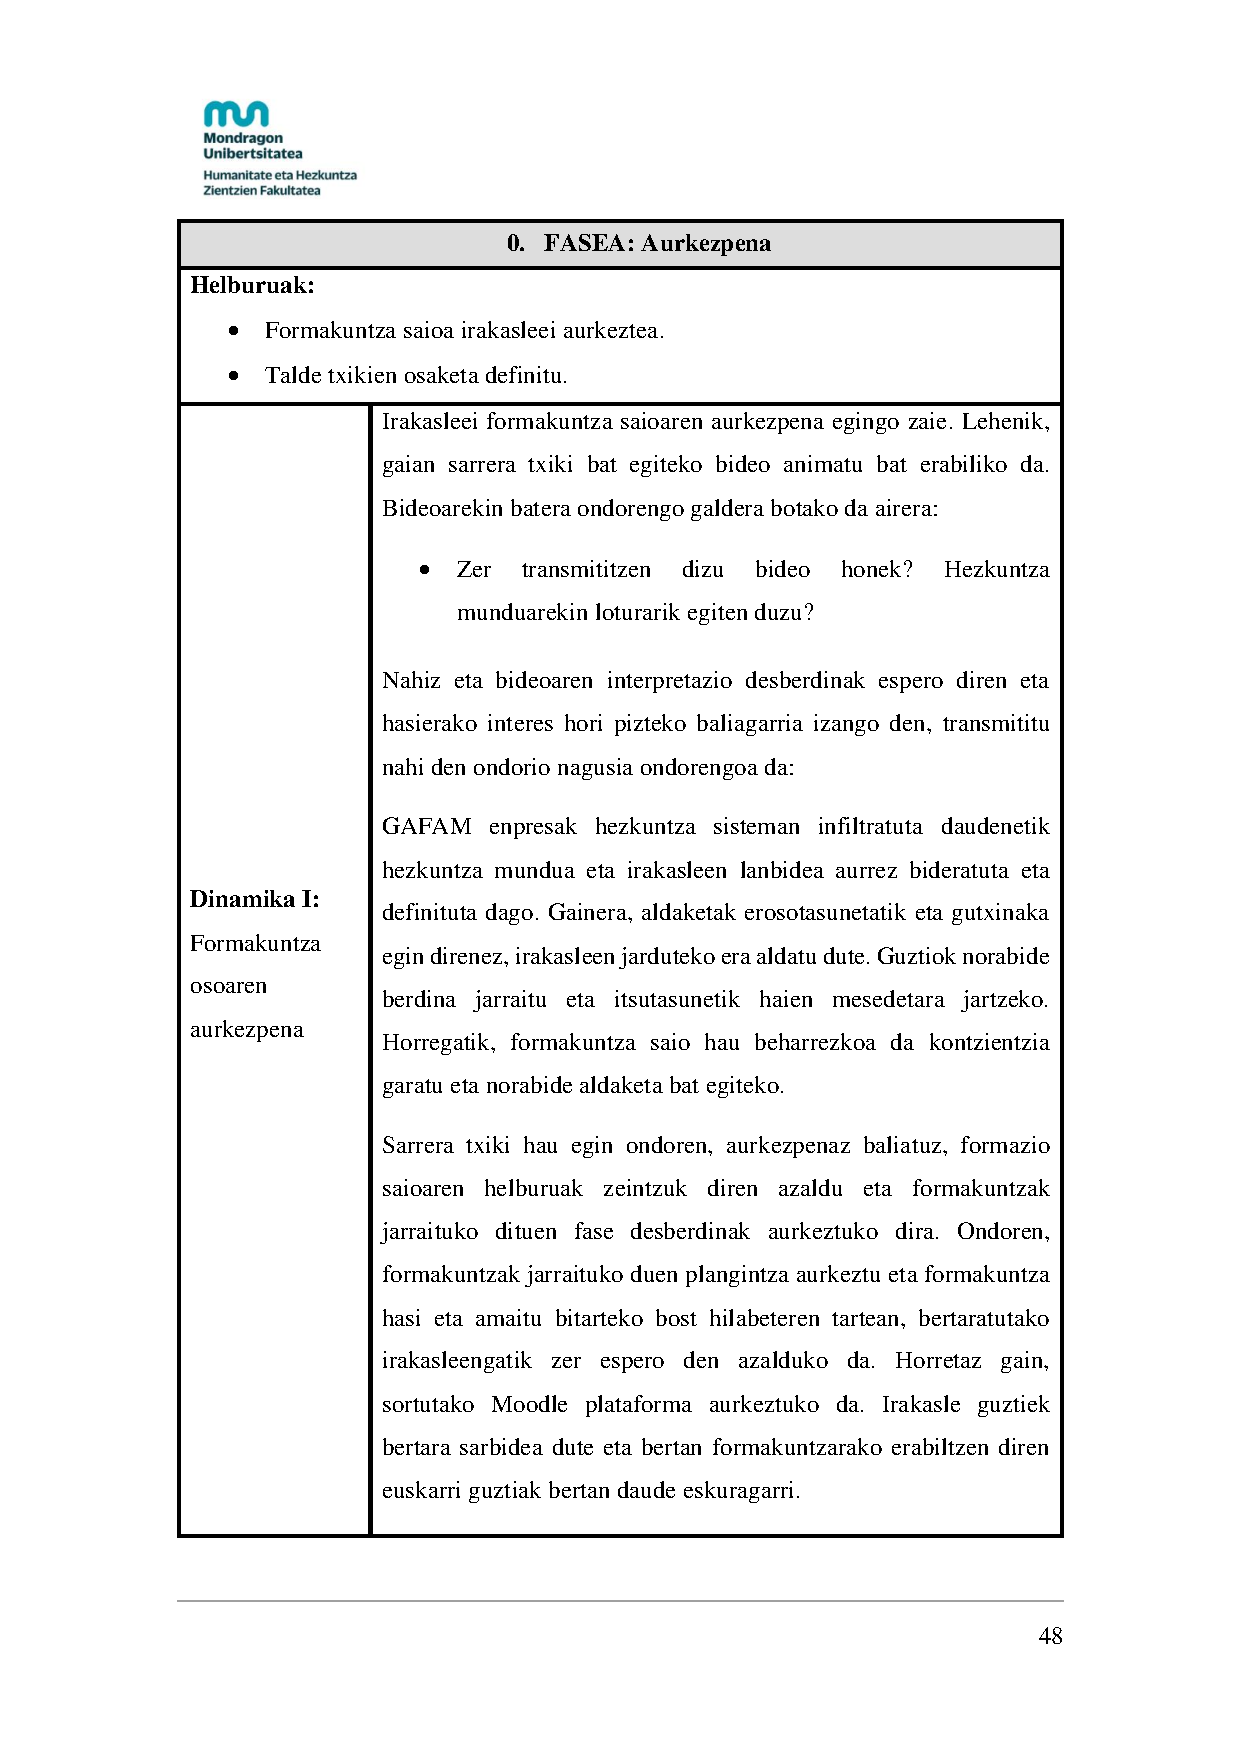
\includepdf[pages=-]{nnapa} %taula egiteko astirik ez dago

\section{Ebaluazioa}
Ebaluazioaren helburua, alde batetik formakuntza bera ebaluatzea da. Formakuntza bera eraginkorra eta dinamikoa izan den, baliabide egokiak erabili diren eta hobekuntzarako tarterik balego, ezaugarri hauek adieraztea da, besteak beste. Azken finean, ikastetxeetan eraginkorra eta baliagarria izango den formakuntza hau, formakuntza jasotzen duten irakasleen feedback eta hobetzekoekin osatzen joatea aberasgarria izango da partaide eta eragile guztientzat. 

Bestetik, formakuntza jasotzen duten irakasleek haien buruaren autoebaluazioa egitea litzateke bigarren helburua. Horretarako, formakuntzan jasotako baliabide eta hausnarketarako espazioak, irakasle jardunean eta gizarte honetako biztanle moduan izan duen eragina neurtzea. Hilabete hauetan zehar, hasierako eta amaierako egoerak kontuan hartuta, egindako prozesuaren kontzientzia hartu eta norberaren burua azaleratutako helburu eta gai desberdinekiko ebaluatzea eta kezkak adieraztea. 

\chapter{Ondorioak}\label{cha:ondorioak}

Txosten honetan, \ref{cha:helburuak}. atalean, finkatu diren helburuak aztertuz, hainbat ondorio atera daitezke. Aldez aurretik, formakuntza saioaren eraginkortasuna aztertzeko testuinguru erreal batean kokatzea (ikastetxe batean martxan jartzea) falta dela aipatu nahi da. Beraz, ondorio hauek zorrozteko, formakuntza saioaren ebaluaketa bat faltako zen.

Lehenik eta behin,  digitalizazio mailaren azterketaren inguruan,  helburua bete dela esan daiteke. DigCompEdu markoa aztertuz, eta EAEko testuinguru digitalaren irudi errealista bat lortu da, ondoren hezkuntzan esku hartzen duten enpresekin erlazionatzeko. Baina, nahiz eta DigCompEdu markoa erabilgarria izan, ez du burujabetza digitalean inolako erreparorik egiten, konpetentzia digitalak bakarrik neurtzen ditu. Hau honela izanda, etorkizun baterako, eta formakuntza saioa hobetzeko asmoz, bestelako ikerketa bat egin beharko litzateke, EAEko irakaslegoaren enpresa handiekiko dependentzia maila aztertzen duena.

Burujabetza mailarekin jarraituz, eta aurrekarietan fokua jarrita, EAEko, Espainiar estatuko eta  Europar mailako burujabetza maila zein den ikusi da, GAFAM enpresek duten eragina aztertuta. Honetaz gain, mugimendu desberdinak aztertu dira, eta hauek duten oinarriak ikertu eta formakuntzan parte hartu dute. Arlo honi dagokionez, formakuntza saioaren helburu nagusia izanda, helburua bete dela esan daiteke.

Amaitzeko, formakuntza saioaren ondorioak bilduko dira. Lehenengo ondorioa honakoa da: ez da DBHko eta batxilergoko irakasleentzat bideratutako formakuntza saioa egin, jarraian azalduko da arrazoia. Formakuntzaren edukiak direla eta,  ezin daiteke esan bi etapa hauetako irakasleentzako formakuntza denik espresuki. Ikastetxeetako burujabetza digitala sustatzean zentratua dagoen saioa denez, etapa hauetatik at ere balio dezake. Baina egia da ere konpetentzia digitalaren garapena, EAEko hezkuntza curriculumean biltzen den bezala, etapa hauetan burutzen dela. Beraz, helburu hau bete den ala ez kontutan izateko orduan, baietz esan daiteke.

Metodologia aktiboei dagokionez, formakuntza saioan gauzatutako dinamiken bitartez metodologia aktiboak erabiltzea sustatu da. Alde batetik, ekipo lanean aritzea bermatu da uneoro, bai talde txiki zein irakasle lantaldeko komunitate moduan. Horretarako, irakaslearen aurre ezagutzak piztu dira saio bakoitzaren hasieran, baliabide digital eta euskarri desberdinak erabiliz formakuntzaren helburu nagusia kontuan hartuta praktika eredugarria izatea bermatu da. Azkenik, bai irakaslearen progresua neurtzeko eta formakuntza saioaren feedback-a jasotzeko ebaluazioak gauzatu dira.

Azken helburu honekin lotuta, formakuntza saioa komunitatea eratzera zentratua izan da. Saioetan burututako ikasketa metodo dinamikoez gain, talde eboluzioan zentratu da, eta saioetatik kanpo ere ikastetxean begirada jarri eta etorkizuneko erronkak kontuan hartuta, ikastetxerako epe luzerako helburuak definitu dira eta hauek gauzatzeko plan bat. Horretarako, irakaslearen ikasketa prozesua bultzatu da, formakuntza saiotik kanpo, sakontzeko baliabideak eskainiz eta irakasle lantaldean jakintzak partekatuz.

Hau dela eta, formakuntza saioa metodologia aktiboetan oinarritua izan dela esan daiteke, eta praktika komunitate bat eratzeko bidea egin duela.

Kurtsoa burujabetza digitalaren inguruko hausnarketa bezala ulertuta, eta baliabide digital libreen erabileraren aldeko testua izanik, hipokresia izango litzateke baliabide ireki hauen erabilerarik ez egitea. Kurtsoa osatzen duen materialaren ehuneko handi bat baliabide irekiak erabiliz sortu da, baina ezin izan da osoki baliabide digital askeetan oinarritu. Dokumentu honetan zehar azaltzen den bezala, norbanakoaren lanak ez dauka eragin handirik, eta komunitate baten laguntza behar da burujabetza hau eskuratzeko. MBL hau, hezkuntza sistemaren parte izanik, ez da bere kabuz baliabide digital libreetan oinarritzeko gai. Helburua ez da bete, baina bi gauza argi geratu dira horrela: multinazionalen menpekotasuna existitzen dela, eta burujabetza digitala talde lanarekin (bai irakasle, bai ikasle eta bai eskolako azpiegitura osatzen duten langile guztien  lanarekin) lortu behar den gauza bat dela.

Bukatzeko, ebaluazioaren inguruko helburuen inguruan, eta berriz ere, praktikan jarri arte ondorio erreal bat ateratzeko jakintzarik izan gabe, bai irakasleen autoebaluaziorako eta bai kurtsoaren feedbackerako tresnak sortu dira. Honekin, irakasleek beraien burua ebaluatu eta formakuntzaren ebaluazio bat egitea espero da, baina ezin daiteke ondorio gehiagorik atera.  

\chapter{Etorkizunerako ildoak}\label{cha:etorkizuna}

Txosten honetan diseinatu eta definitzen den irakasleentzako formakuntzak eta orokorrean landu den Master Bukaerako Lan honek, etorkizunera begira hainbat lan lerro ireki eta garatzeko aukera eskaintzen du, gaur gaurkoz denbora mugatu izan baitu lan hau burutzeko. Etorkizunean garatzeko aukera duten lan ildoei dagokienez, lehenik eta behin, formakuntza saio hau ikastetxean gauzatzen den momentuan eta irakasleek bukaeran betetzen duten ebaluazio taula kontuan edukiz, hainbat hobekuntza aplikatu beharko lirateke. Etengabeko hobekuntza ardatz edukiz, beste ikuspegi batzuk kontuan hartuz, geroz eta formakuntza eraginkorrago bat lortzeko.

Horrez gain, formakuntza saio honen bitartez lortu nahi dena hezkuntzan erabiltzen diren baliabide digitalen erabilera kritiko bat egitea eta aldi berean, irakaslegoa baliabide digital libreetan trebatzea, ondoren ikasgelan erabiltzeko. Horregatik, formakuntza saioan eskuratutako jakintza horiek guztiak aurrera begira ikastetxe guztira zabaltzea ezinbestekoa da. Alde batetik, irakasleei baina baita ere guraso, zuzendaritza eta ikasleei, hau da, ikastetxeko hezkuntza komunitate osoari.
Bertatik, lan- talde bat sortu beharko litzateke prozesu honen gidaritza hartuko lukeena eta ez soilik pertsona batengan erortzea ardura guztia, nahiz eta ikastetxeko partaideen ardura izan arlo honen eraldaketa.

Modu horretara, komunitate osoa inguratzen dituen errealitatearen kontzientzia hartuta, hurrengo pausua ikastetxeko diagnosi sakon bat egitea izango litzateke, formakuntza saioan egingo diren behaketa taulak eta profil ezberdinetako iritziak kontuan hartuta. Behin, diagnosia oinarri hartuta, egungo errealitatea irauli eta burujabetza digitalerako bidean, bide- orri bat diseinatu beharko litzateke hurrengo pausuak definitzeko. Horretarako, garrantzitsua izango litzateke baliabide digital libreak sortzen dituzten enpresekin kontaktuan jartzea, proposamen pertsonalizatuak diseinatzeko ondoren ikastetxean txertatzeko eta horien erabilera egoki bat egiteko formakuntza eskaintzeko.

Honetaz guztiaz gain, beharrezkoa ikusten da irakasleen konpetentzia digitalen maila aztertzeaz gain (DigCompEdu markoan oinarrituz), hauen burujabetza digital maila analizatuko duen azterketa bat gauzatzea, bertatik informazio oso baliagarria eskuratuko delako egungo errealitatea ulertzeko eta etorkizunean martxan jarri beharreko proiektuak definitzeko.



%----------
%	BIBLIOGRAFIA
%----------

% \nocite{*} % Bibliografiara gehituta dauden dokumentu guztiak azaltzeo (nahiz eta ez erabiliak izan), kendu lerro honen aurretik dagoen %

\clearpage
\printbibliography[heading=bibnumbered, title=Bibliografia]

%----------
%	ERANSKINAK
%----------
% Lanak eranskinik baditu, aktibatu hemengo zati hau
\appendix
\chapter*{Eranskinak}
\addcontentsline{toc}{chapter}{Eranksinak}
%\pagenumbering{gobble} % eranskinak ez dira numeratzen
\renewcommand{\thesection}{Eranskina \Roman{section}}
\section{Moodle plataformaren erabilera baldintzak}\label{eranskin:moodle}
Moodle plataforma libre bat da, eta norberak zerbitzari pribatu batean montatu behar du. Bestalde, interneteko domeinuak ere ordainpeko plan batera daude lotuak.

Hau horrela izanda, “burujabetzadigitala.eus” domeinua Mondragon Unibertsitateak PuntuEUS fundazioarekin duen eskaintza erabiliz eskuratu da, non 364 egunerako domeinu bat doan erregistratu daitekeen, ikasle izanez gero. Hori dela eta, ez da bermatzen 2023ko ekainaren 11tik aurrera sarbidea izaterik \url{http://burujabetzadigitala.eus/moodle} linka erabiliz. Zerbitzari hau islatuta dago “sampru.ovh” domeinuan, beraz, behin aurreko data igaro eta gero, posible da Moodle plataforma \url{http://sampru.ovh/moodle} helbidean eskuragarri izatea.

Aldi berean, zerbitzaria erabilera pribaturako da. Beharra izanez gero, Moodle plataforma kendu egingo da beste proiekturen bat garatzeko. Honekin adierazi nahi dena da ez dagoela inolako bermerik dokumentu hau irakurtzen ari den unean euskarri digital hau erabili ahal izateko.

Dena den, eta tesiaren formakuntza saioaren inguruko materiala eskuratu nahi baduzu, gunearen segurtasun kopia bat eskuragarri egongo da ondorengo \href{https://drive.google.com/drive/folders/1S8kl20k8nW0w-bopBuNT5HyozOxtO4Ei?usp=sharing}{linkean}.

% Kontraportada
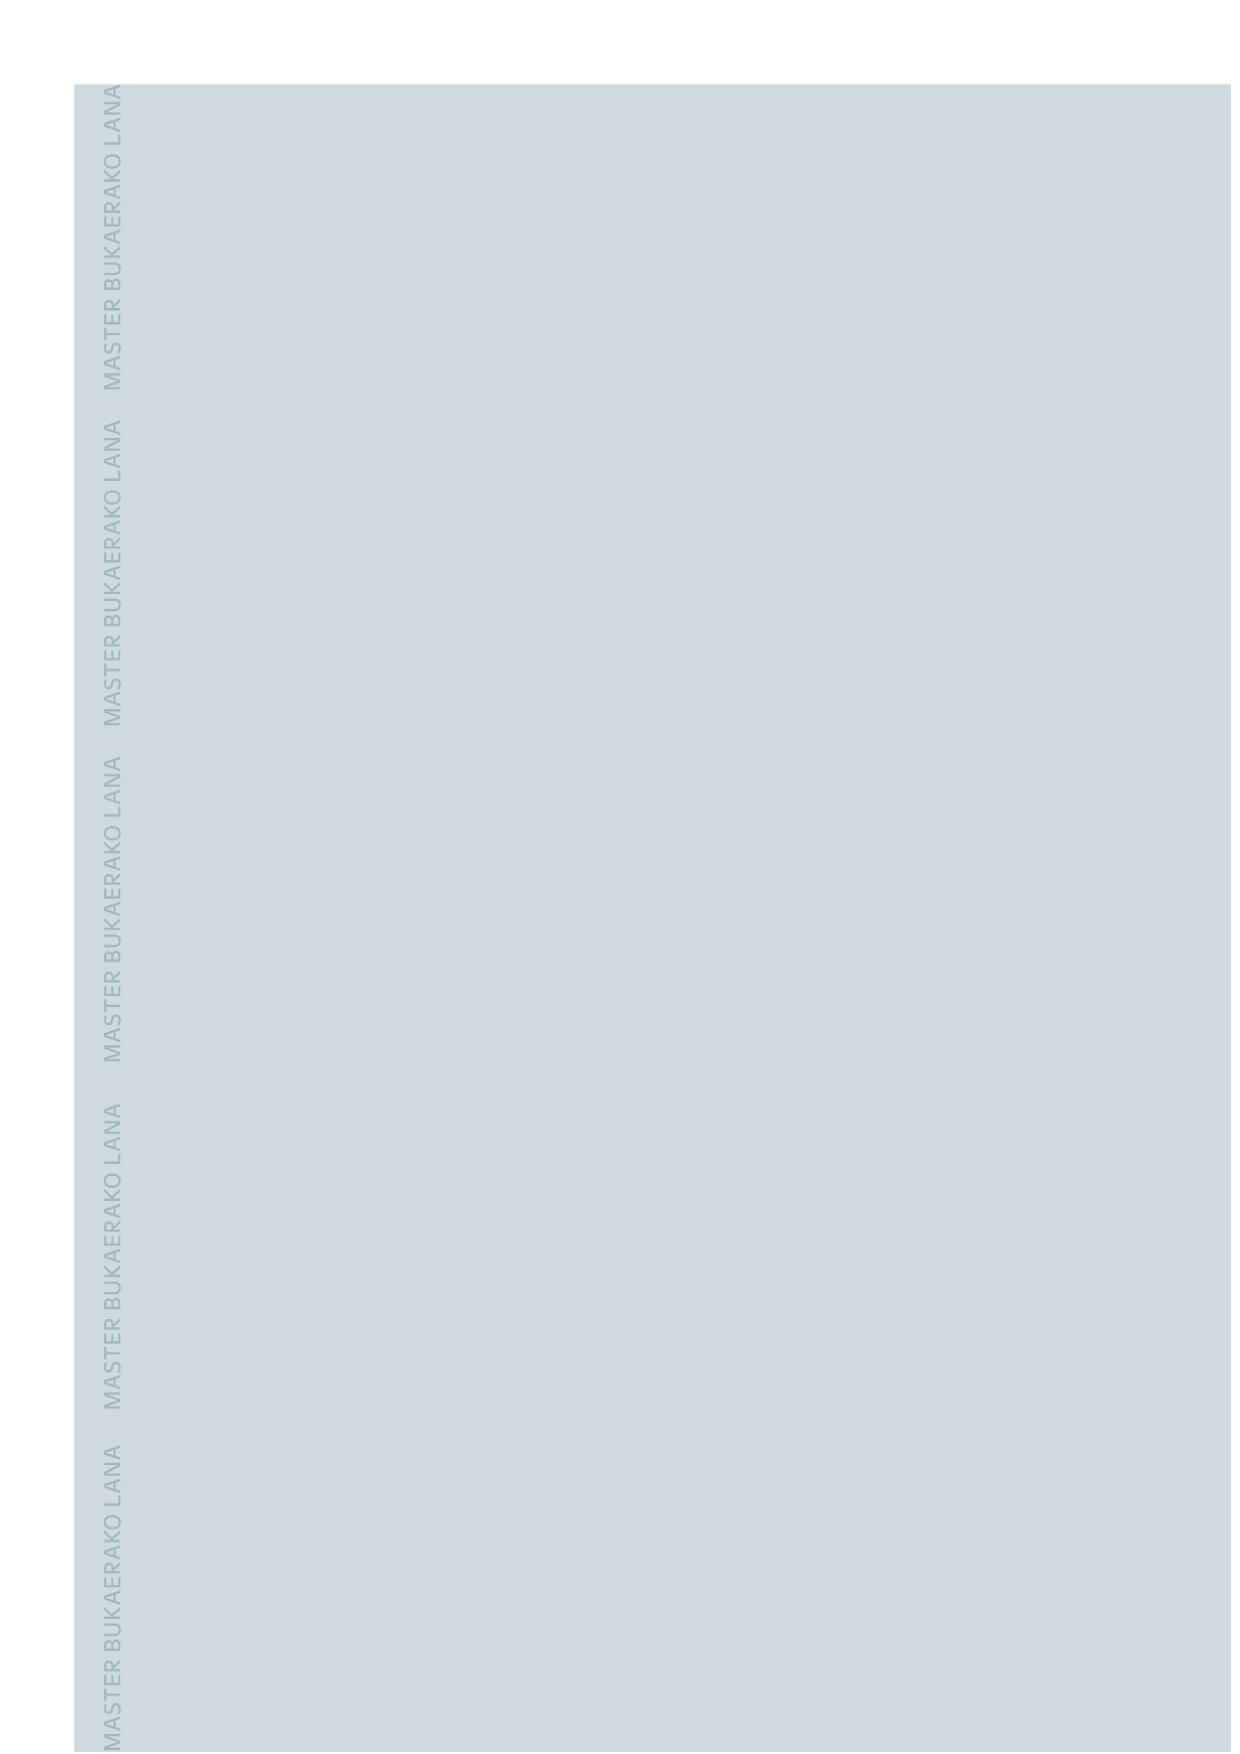
\includepdf[pages=-]{resources/Kontraportada}
\end{document}
